%
% This program is free software: you can redistribute it and/or modify
% it under the terms of the GNU General Public License as published by
% the Free Software Foundation, either version 3 of the License, or
% (at your option) any later version.

% This program is distributed in the hope that it will be useful,
% but WITHOUT ANY WARRANTY; without even the implied warranty of
% MERCHANTABILITY or FITNESS FOR A PARTICULAR PURPOSE.  See the
% GNU General Public License for more details.

% You should have received a copy of the GNU General Public License
% along with this program.  If not, see <http://www.gnu.org/licenses/>.

\documentclass{book}

\usepackage{mystyle}

\title{R 스터디 가이드 \\
   - 도움이 되길 바랍니다 - 
   }
\author{iHELP Working Group \\ Chel Hee Lee \& Eugene Jung } 
\date{\today}

\begin{document}
\maketitle

%%%%%%%%%%%%%%%%%%%%%%%%%%%%%%%%%%%%%%%%%%%%%%%%%%%%%%%%%%%%%%%%%%%%%%%%
%
%
% PART I
%
%
%%%%%%%%%%%%%%%%%%%%%%%%%%%%%%%%%%%%%%%%%%%%%%%%%%%%%%%%%%%%%%%%%%%%%%%%

\part{R을 처음 접하는 분들을 위하여}

% \chapter{시작하면서}

통계소프트웨어 \texttt{R}을 사용하는데 이 문서가 도움이 되길 바랍니다. 
아래와 같은 내용에 중점을 두고자 하였습니다. 

\begin{itemize}
\item 원리중심의 문제해결을 설명하고자, 다양한 패키지들로부터 제공되는 함수들에 대한 사용법에 대한 설명은 가급적이면 피하려고 하였습니다.
따라서, 이 문서내에서는 특정 패키지가 해결할 수 있는 경우를 제외하고는 BASE (기본) 시스템을 이용하여 문제를 해결할 수 있도록 정리하려고 노력합니다.

\item R이라는 언어의 특징을 살린 설명을 하고자 하였습니다.  
예를들면, R의 가장 큰 특징이라고 할 수 있는 벡터라는 개념을 활용하여 원리 중심의 설명을 제공합니다. 

\item 통계와 전산에 관련된 전문용어는 쉽게 풀어쓰거나, 용어에 대한 이해를 돕기 위한 참고 자료를 제공합니다. 
\end{itemize}

본 문서와 관련한 프로젝트의 시작일은 2013년 4월 10일이며, iHELP Working Group 관리자에 의하여 수시로 갱신되고 있습니다.
따라서, 이 문서는 어떤 특정한 기간을 두고 완성되지 않으며, 오로지 업데이트된 버전만이 존재합니다.

이 문서는 2005년 이래로 R의 사용에 대한 본 문서의 지은이 개인의 경험과 R Documentation 만을 토대로 하여 작성되었으므로 아직 경험하지 못하여 다루지 못하는 부분이 있습니다.
이 문서의 지은이는 통계학에 대한 
%  B.Sc. (Statistics), M.Sc. (Statistics), 그리고 PhD. Biostatistics Candidate 의 
배경지식을 가지고 있으므로 문서의 내용이 다소 통계 및 수학 분야에 치중하였을 수 있습니다.
지은이는 이 문서가 보다 다양한 계층의 분들께서 R을 이용하여 하고자 하시는 일에 밑거름이 될 수 있는 도움이 되고자 합니다.
따라서, 이 문서를 읽고 있는 독자가 문서 내용에 대한 추가, 수정, 및 제안이 있다면 \href{mailto:gnustats@gmail.com}{gnustats@gmail.com} 또는 \href{mailto:ihelp-urquestion@lists.r-forge.r-project.org}{ihelp-urquestion@lists.r-forge.r-project.org} 의 주소로 이메일을 보내주신다면 감사하겠습니다. 

또한, 아래에 기재된 분들 (가나다 순)의 관심과 제안들이 없었다면 이 문서가 발전될 수 없었기에 그 감사의 말씀을 올리고 싶습니다. 
\begin{itemize}
\item 신종화 교수님 (서울종합과학대학원 사회학과)
\item 이부일 박사님 (충남대학교 정보통계학과)
\item 정우준 박사님 (홍익대학교 경영학과)
\item 
% \item 이영섭 교수님 (동국대학교 통계학과)
\end{itemize}

\paragraph{이 문서를 읽는 방법:} 
\begin{itemize}
\item ``완전초보에요''라는 챕터와 ``기초프로그래밍과 운영체제'' 챕터는 이 문서를 읽기 전에 반드시 먼저 읽으셔야 합니다.  
\end{itemize}

%%%%%%%%%%%%%%%%%%%%%%%%%%%%%%%%%%%%%%%%%%%%%%%%%%%%%%%%%%%%%%%%%%%%%%%%
%
%
%
%%%%%%%%%%%%%%%%%%%%%%%%%%%%%%%%%%%%%%%%%%%%%%%%%%%%%%%%%%%%%%%%%%%%%%%%

\chapter{완전 초보에요}

이 문서에서 ``초보''라는 의미는 아래에 나열된 사항들중 두 가지 이상에 해당되시는 분들을 의미합니다. 

\begin{itemize}
\item R 이라는 프로그래밍 언어 이전에 다른 프로그래밍 언어에 대한 경험이 전무하신 분,
\item 유닉스와 리눅스 시스템에 익숙하지 않으신 분,
\item 기초 통계 분석에 대한 도움이 필요하신 분,
\item 그냥 무엇을 해야할지 막막함에 쌓여 계신분 
\end{itemize}

이에 해당하시는 분들은 꼭 ``사용전 반드시 알아야 할 7가지 숙지사항'' 섹션을 꼭 읽어주시길 부탁드립니다.
R을 사용하시는데 있어 숙지사항의 내용을 기억하신다면, 매우 도움이 될 것입니다. 


%%%%% SECTION START 
\section{꼭 먼저 알아야 할 7가지}

초보라고 생각하시는 분들께서는 아래의 내용들에 미리 알고 계시면 R을 사용하는데 도움이 됩니다.

\begin{enumerate}
  \item  \textbf{데이터 입력과 처리:}  R 에서는 이용되는 모든 데이터들에 대한 처리는 열방향으로 이루어집니다.
이 말의 뜻은 데이터의 입력 및 변형, 그리고 연산에 사용되는 데이터들에 대한 처리순서는 열방향으로 나열된 후에 이루어지는 것을 말합니다. 
예를들어, 1부터 12까지 12개의 정수로 이루어진 수열 (즉, $\{ 1, 2, 3, 4, 5, 6, 7, 8, 9, 10, 11, 12 \}$)을 수학적인 표현으로 4행 3열의 행렬은 R은 아래와 같이 이해합니다. 

% 데이터 불러오기
% 보통 사람들은 R 콘솔에서 직접 입력한 데이터를 제외하고 그 외의 데이터는 *.txt, *.xlsx 이든 *.sav이든 모두 외부데이터로 생각하기
% 일쑤이다.
% 즉 foreign 팩키지를 사용해야 하는 경우를 제대로 구분하지 못한다. 그러니,
% > library(foreign)
% 을 선언할 줄 모르는 것은 당연하다.

% 그리고 인코딩이란 무엇인지를 모르는 사람은 보다 맞다.

\begin{Schunk}
\begin{Soutput}
1  5   9
2  6  10
3  7  11
4  8  12
\end{Soutput}
\end{Schunk}

따라서, 이 행렬에서 5라는 숫자값은 행렬의 1행 2열에 위치하고 있다고 할 수 있으며, 행렬의 5번째의 값이라고도 할 수 있습니다. 

  \item  \textbf{대화식 사용과 결과를 보는 방법에 대해서:} R은 사용자가 주어지는 업무를 시키는 대로만 수행하는 유용한 프로그램일뿐, 그 이상의 내용은 수행하지 않는다는 점을 반드시 명심하셔야 합니다. 
따라서, R 프로그램을 시작하게 되면 아래와 같은 기호로 표시되는 프롬프트 (즉, 사용자의 명령어를 기다리는 기호)를 보여주게 됩니다. 
\begin{Schunk}
\begin{Soutput}
>
\end{Soutput}
\end{Schunk}

모든 명령어는 $>$ 기호 뒤에 작성하게 됩니다. 

가장 중요한 것은 분석자가 머릿속으로 상상하거나 기대하는 업무가 있다면, 분석자는 반드시 그 업무가 이루어지는 프로세스에 대해서 잘 알고 있어야 합니다.
따라서, R은 다른 통계 소프트웨어들과 같이 분석된 결과를 미리 보여주거나 혹은 분석이 된 모든 결과를 한 번에 다 보여주지 않습니다.
분석자가 확인하고자 하는 결과를 R에서 제공하는 함수를 통하여 중간 결과물들을 확인할 수 있습니다. 
우리는 분석자가 작업을 어떻게 진행하고 확인할 것인가에 대한 프로세스 차트를 먼저 작성한뒤 분석을 수행하기를 권장합니다.


  \item \textbf{통계분석의 절차:} 분석이라 것은 데이터에 대한 이해를 통하여 데이터가 가진 특징을 수학적 표현으로서 설명하기 위한 과정입니다. 
따라서, 데이터에 대한 직관적인 이해를 위해서 시각화 작업과 통계 모형이 요구하는 데이터 형식을 만드는 것이 중요합니다. 
이를 전처리 과정이라고 하며, 통계분석은 크게 아래와 같은 절차를 밟아 이루어집니다.

\begin{itemize}
\item 데이터 입출력과 클리닝, 그리고 분석 전처리 관련 테크닉들
\item 분석전 탐색적 시각화 작업 
\item 통계모형의 결정 및 적용 
\item 모형 적용 후의 보고서 생성 및 시각화 작업
\item 통계 모형 자체의 개발 또는 자동화 시스템 구축
\end{itemize}

따라서, 이 문서는 위에서 설명한 과정에 해당하는 순서대로 챕터들을 구성하였습니다. 


  \item \textbf{한글 표현과 인코딩에 관련하여:}


  \texttt{R}은 한국어 사용자를 위한 한국어 인터페이스를 지원하고 있습니다. 
\textbf{그러나, 사용자는 이러한 한국어 지원이 단순히 사용자의 편의를 위한 선택적 사항이라는 점을 반드시 알고 있어야 합니다}.
또한, 분석시 본래의 정교한 표현은 번역된 한국어 보다는 원래의 영문이라는 점도 잊지 마셔야 합니다. 

현재 한국어에 관련된 작업은 UTF-8이라는 인코딩에 기반하여 한국어 품질관리 프로그램 (\url{http://ihelp.r-forge.r-project.org/lang_msg.html})을 통하여 이루어 지고 있으나, \texttt{R}을 한국어가 아닌 영문으로 설정하기 위해서는 다음의 주소를 눌러 그 내용을 확인해주시길 부탁드립니다. 
이 내용은 버전에 관계없이 일반적으로 통용되는 방법이나 윈도우즈 사용자에게 맞추어 작성되었습니다. 

\url{http://lists.r-forge.r-project.org/pipermail/ihelp-urquestion/2013-April/000003.html}

본래 데이터를 자국의 언어로 표현하는 방법은 UTF-8 이라는 인코딩을 이용하므로, 간혹 데이터가 올바르게 보이지 않을 경우가 있습니다. 
이러한 문제를 해결하기 위해서는 ``R을 지원하는 인코딩 중 올바르게 한국어를 표현해주는 코드를 찾는 방법'' (\url{http://lists.r-forge.r-project.org/pipermail/ihelp-urquestion/2013-April/000017.html}) 를 읽어보시길 바랍니다.

간혹, 잘못된 한글처리가 시스템 에러를 야기하는 경우가 있으므로, 이러한 경우에 한국어로 R을 사용하시는 분들께서는 다소 번거로우실지라도 보다 안정적이고 나은 R을 제공하기 위하여 그 내용을 \href{mailto:ihelp-urquestion@lists.r-forge.r-project.org}{ihelp-urquestion@lists.r-forge.r-project.org} 주소로 이메일을 보내주신다면 감사하겠습니다. 

단, 이러한 한글처리는 분석에 연관된 수치연산과는 아무런 관계가 없음을 반드시 알아주시길 부탁드립니다.


	\item \textbf{대소문자 구분에 관련하여:}
많은 분들이 이전에 SAS 소프트웨어를 사용하여 분석을 수행하셨을 것입니다.
SAS에서는 대소문자를 구분하지 않고 프로그램을 작성하게 되지만, R에서는 대소문자를 구분하므로 A 라는 변수와 a 라는 변수는 서로 다른 것임을 명심하시길 부탁드립니다. 


	\item \textbf{운영체제와 관련하여:}
R은 기본적으로 Unix (유닉스)와 같은 환경에서 작성되었습니다. 


	\item \textbf{함수의 사용에 관련하여:}  R보다도 일반적으로 프로그래밍을 다소 익숙하게 다룬다는 것은 하고자 하는 업무에서 어떤 함수가 적재적소에 쓰여야 할 지를 아는 것입니다. 
	따라서, 제공되어지는 함수가 무엇이 있으며 어떤 함수가 언제 어떻게 사용되는가를 알고 있는 것은 작업하는데 도움을 줍니다. 
	함수를 사용할 때,  R은 네임드 아규먼트과 함께 사용하는 것이 좋습니다.  

	\item \textbf{패키지와 관련하여: }
R은 Add-on이라는 패키지 시스템을 이용합니다. 
이것은 기본 베이스 시스템에 추가로 필요한 기능들을 추가하는 의미입니다.
이러한 내용을 잘 모르는 상태에서 초보자가 가장 많이 겪는 실수는 어떤 함수를 사용하고자 할 때 ``xxx 함수가 없습니다'' 또는 ``xxx 함수를 찾을 수 없습니다''입니다.
이는 사용하고자 하는 함수가 R 기본 배포판에 포함되어 있지 않은 어떤 사용자에 의해서 제공된 특정한 패키지내에서 존재하기 때문입니다.
이런 경우에는 먼저 사용하고자 하는 함수가 어떤 패키지에 존재하는지 알아야 합니다.  
그리고, 해당 패키지를 설치했을 때에는 설치된 패키지를 사용할 수 있도록 로딩하는 과정을 거쳐야 합니다.

\begin{Schunk}
\begin{Soutput}
> library(pkg_name)	
\end{Soutput}
\end{Schunk}

패키지의 설치, 확인에 관련된 사항은 ``통계모형의 선택과 적용''이라는 챕터에 기록해두었습니다. 

\end{enumerate}


%%%%% SECTION START 

\section{왜 R을 사용하나요?}

R을 사용하는 이유는 아마도 아래와 같은 이유이기 때문입니다. 
(R Documentation에는 없는 이 문서의 지은이 개인의 생각임을 명심하시길 바랍니다)

\begin{enumerate}
	\item R은 매우 다양한 분야에서 개발되고 적용되는 최신 통계기법을 적용할 수 있는 자유소프트웨어이기 때문입니다.
	\item 행렬기반의 객체지향적 프로그래밍 언어이기 때문입니다.
	\item 다른 소프트웨어들에 비교하여 문법적 사용의 자유롭기 때문일 것입니다.
\end{enumerate}


\section{통계소프트웨어의 종류}

R이라는 통계소프트웨어를 대체할 수 있는 다른 소프트웨어들은 다음과 같습니다. 

\begin{itemize}
\item S-PLUS (상업용 버전의 S 언어 소프트웨어)
\item MATLAB (R과 같은 행렬기반의 언어)
\item SPSS
\item Octave (MATLAB의 GNU 버전)
\item Python (프로그래밍 언어)
\item SAS
\item STATA
\end{itemize}
% Gretl


%%%%%%%%%%%%%%%%%%%%%%%%%%%%%%%%%%%%%%%%%%%%%%%%%%%%%%%%%%%%%%%%%%%%%%%%
%
%
%
%
%
%%%%%%%%%%%%%%%%%%%%%%%%%%%%%%%%%%%%%%%%%%%%%%%%%%%%%%%%%%%%%%%%%%%%%%%%

\chapter{사용환경에 익숙해지기}

R은 연구활동의 수행을 위한 도구일 뿐입니다. 
이 도구를 잘 활용한다는 것은 그만큼 주어진 사용환경에 익숙해져 있다는 의미와 같습니다.
따라서, 본 챕터에서는 R을 처음에 접하는 사용자들이 R이라는 작업도구를 사용함에 익숙해지도록 먼저 계산기능으로서의 측면을 벡터, 행렬, 그리고 배열이라는 것을 통하여 먼저 살펴보도록 하겠습니다.
이들을 설명하는 이유는 추후에 다루어질 모든 내용들이 이것들과 관계가 있기 때문입니다. 


\section{R의 시작과 종료}

먼저 R을 시작하면 아래와 같은 화면을 볼 수 있습니다.

\begin{Schunk}
\begin{Soutput}
R version 2.15.1 (2012-06-22) -- "Roasted Marshmallows"
Copyright (C) 2012 The R Foundation for Statistical Computing
ISBN 3-900051-07-0
Platform: i686-pc-linux-gnu (32-bit)

R is free software and comes with ABSOLUTELY NO WARRANTY.
You are welcome to redistribute it under certain conditions.
Type 'license()' or 'licence()' for distribution details.

  Natural language support but running in an English locale

R is a collaborative project with many contributors.
Type 'contributors()' for more information and
'citation()' on how to cite R or R packages in publications.

Type 'demo()' for some demos, 'help()' for on-line help, or
'help.start()' for an HTML browser interface to help.
Type 'q()' to quit R.

> 
\end{Soutput}
\end{Schunk}

그리고, $>$ 라는 기호 바로 뒤에 깜빡깜빡 거리는 커서를 볼 수 있을 것입니다. 
이것은 R이 사용자의 입력을 기다린다는 의미입니다. 
이 기호를 프롬프트라고 하고, 프롬프트 기호 바로 뒤에서부터 명령어를 작성합니다. 

사용자의 명령이 끝났음을 알려주는 것이 엔터키입니다. 
R이 입력된 명령어를 처리하여 사용자에게 명령어의 수행 결과를 보여주는 것은 아래와 같습니다.
이는 항상 $[1]$ 이라는 기호로 시작합니다. 
실제로 $[1]$ 이라는 것은 추후에 설명하겠지만 첫번째 객체를 의미하는 것입니다.

\begin{Schunk}
\begin{Soutput}
> 1
[1] 1
> 1+1
[1] 2
\end{Soutput}
\end{Schunk}

이렇게 사용하는 방식을 R 소트트웨어와 대화식으로 사용한다고 하며, 이러한 대화가 이루어지는 공간 (즉, 사용자가 R에게 질의응답을 하는 곳)을 콘솔이라고 합니다.

작업을 다 한 뒤에 종료를 하고자 한다면 q() 명령어를 이용하여 R의 사용을 종료할 수 있습니다. 

\begin{Schunk}
\begin{Soutput}
> q()
Save workspace image? [y/n/c]: n
\end{Soutput}
\end{Schunk}

이때 workspace image (작업공간의 이미지)를 저장하겠는가라는 메시지를 보게 될 것입니다. 
작업공간 이미지라는 것은 콘솔내에서 현재 세션에서 작업을 해온 명령어들의 기록과 데이터들을 보관하겠는가에 대한 질문입니다. 

\section{1차원 벡터와 벡터라이제이션}

R의 가장 큰 특징은 모든 연산에 관련된 기능들이 벡터방식으로 동작하는 것을 의미합니다. 
벡터라는 개념은 컴퓨터가 어떠한 임의의 것을 1차원에서 다루는 것을 의미합니다.
예를들어, 수학에서 1이라고 표시하는 것을 컴퓨터가 알아듣게 입력을 한다면 단순히 1 이라는 값만을 입력하면 됩니다. 
그러나, 실제 작업에서 우리는 동일한 연산을 반복해야 하는 경우가 있습니다. 
따라서, 숫자 1이 아닌 1, 3, 5, 7, 9 와 같은 여러개의 숫자들을 나열한 수열의 형태를 만듭니다. 
이제, 1,3,5,7,9는 수열의 구성요소가 되는 것입니다. 
이러한 수열의 표현방식을 R이 알아듣도록 하는 것을 우리는 벡터라는 개념이라고 이야기 합니다. 

벡터방식이란 개념을 이해하기 위해서 계산기로서 R은 어떤 기능을 가지고 있는지 먼저 이해해야 합니다.

\subsection{산술연산}

먼저 R은 아래와 같은 사칙연산 (더하기, 빼기, 곱하기, 나누기)이 가능합니다. 

\begin{equation}
1 + 2 - 3 + 4*5 - 6/3
\end{equation}

이를 R로 수행하기 위해서는 다음과 같이 입력합니다. 

\begin{Schunk}
	\begin{Soutput}
> 1 + 2 - 3 + 4*5 - 6/3
[1] 18
	\end{Soutput}
\end{Schunk}

연산자라는 것은 어떤 특정 역할을 수행하는 기호이며, 산술연산에 대한  연산자 우선순위는 수학적 연산순서와 동일합니다. 
다음과 같은 다양한 수학적인 연산이 가능합니다. 

\begin{Schunk}
	\begin{Soutput}
> # 제곱 
> 3^2
[1] 9
>
> # 지수 
> exp(3)
[1] 20.08554
> 
> # 로그 
> log(3)
[1] 1.098612
> 
> # 파이상수 값 
> pi
[1] 3.141593
>
> # 삼각함수 사인, 코사인, 탄젠트  
> sin(0)
[1] 0
>
> cos(0)
[1] 1
>
> tan(45)
[1] 1.619775
> 
> # 몫과 나머지 구하기 
> 15/4
[1] 3.75
> 15 %/% 4
[1] 3
> 15 %% 4
[1] 3
> 15 %% 3
[1] 0
> 15 %% 2
[1] 1
> 
\end{Soutput}
\end{Schunk}

이제 R의 벡터단위의 연산이라 것을 알아보도록 합니다. 

먼저 아래와 같이 1, 2, 3, 4 라는 각각의 숫자들을 하나로 묶어 하나의 벡터 (즉, 수열)을 생성해보도록 합니다. 
이때, 이렇게 숫자들을 하나로 묶어 주는 것은 c()라는 함수를 통하여 이루어지게 됩니다.

\begin{Schunk}
\begin{Soutput}
> c(1,2,3,4)
[1] 1 2 3 4
\end{Soutput}
\end{Schunk}

그런데, 매번 이렇게 숫자들의 묶음을 일일이 손가락으로 입력해야 한다면 사용이 매우 번거로울 것입니다. 
그래서 R은 이러한 입력을 임시적으로 저장을 해주는 변수라는 기능을 제공합니다. 
아래와 같이 내가 묶은 일련의 숫자들을 x 라고 불리는 변수에 저장을 하겠다는 의미입니다.
이를 c(1,2,3,4)라는 벡터를 x에 대입 또는 할당한다고 말합니다.
따라서 이제부터는 변수 x를 입력하기만 하면 위에서 입력한 일련의 숫자들이 기억되고 있다는 것을 확인할 수 있습니다. 

\begin{Schunk}
\begin{Soutput}
> x <- c(1,2,3,4)
> x
[1] 1 2 3 4
\end{Soutput}
\end{Schunk}

위에서 할당을 $<-$ 기호를 사용하였으나, 이러한 할당은 아래와 같은 방법으로도 가능합니다. 

\begin{Schunk}
	\begin{Soutput}
> x <- c(1,2,3,4)
> x
[1] 1 2 3 4
> c(1,2,3,4) -> x
> x
[1] 1 2 3 4
> x = c(1,2,3,4)		
> x
[1] 1 2 3 4
\end{Soutput}
\end{Schunk}

이는 단순히 사용자의 편의를 위한 것뿐이니 마음에 들어하는 방식을 골라서 사용하시면 됩니다. 

이제 R이 정말로 x라는 것을 벡터로 인식하는지 is.matrix()라는 함수를 사용하여 알아보도록 합니다. 

\begin{Schunk}
\begin{Soutput}
> is.vector(x)
[1] TRUE
\end{Soutput}
\end{Schunk}

한개의 숫자와 하나의 벡터를 구분짓는 특징은 몇개의 숫자들이 한데 묶였는가 이므로 이를 확인하기 위해서는 length()라는 함수를 사용합니다. 

\begin{Schunk}
\begin{Soutput}
> length(x)
[1] 4
\end{Soutput}
\end{Schunk}

\paragraph{벡터단위의 연산}  이제 벡터단위의 연산이 무엇인가 알아보도록 합니다. 
위에서 생성한 x 라는 변수에 3 을 더해봅니다. 
이때, 우리는 상식적으로 x라는 변수에 있는 벡터를 구성하는 모든 구성요소에 3이 더해진 결과를 볼 수 있기를 기대합니다. 

\begin{Schunk}
\begin{Soutput}
> x+3
[1] 4 5 6 7	
\end{Soutput}
\end{Schunk}

이제 x라는 벡터에 제곱을 해봅니다. 
여러분들은 벡터의 각 구성요소의 값들이 제곱이 되었음을 알 수 있습니다. 
\begin{Schunk}
\begin{Soutput}
> x^2
[1]  1  4  9 16
\end{Soutput}
\end{Schunk}

이번에는 10으로 나누어 보겠습니다.

\begin{Schunk}
\begin{Soutput}
> x/10
[1] 0.1 0.2 0.3 0.4
> 
\end{Soutput}
\end{Schunk}

이렇게 어떤 벡터에 특정 주어진 연산을 수행하고자 할때 벡터의 각 구성요소에 주어진 연산이 한 번에 모두 수행되는 것을 바로 벡터단위의 연산이라고 합니다. 
이를 좀 더 멋있게 부르는 말이 어떤 연산에 대한 벡터라이징이라고 하는 것입니다. 


\subsection{벡터를 생성하는 다양한 방법들}

위에서는 단순히 c()라는 함수를 이용하여 벡터를 생성하였으나, R은 다양한 보다 다양한 방법을 제공하고 있습니다. 

\paragraph{seq()함수의 사용} 먼저 아래와 같이 사용되는 seq()라는 함수가 있습니다. 

\begin{Schunk}
\begin{Soutput}
> seq(0, 1, 0.1)
 [1] 0.0 0.1 0.2 0.3 0.4 0.5 0.6 0.7 0.8 0.9 1.0
\end{Soutput}
\end{Schunk}

위에서 사용한 명령어는 0과 1 사이에 0.1 을 단위로 하는 시퀀스(즉, 수열)을 생성하라는 명령어입니다. 

여기에서 R을 사용하는 한가지 팁을 알려주고자 합니다.
seq() 함수의 예제와 같이 사용하고자 하는 함수에는 여러가지 입력받는 인자들이 있습니다. 
입력되는 인자들의 순서가 틀려진다면 R은 잘 못된 결과를 줍니다. 
따라서, 이러한 실수를 줄이고자 함수를 사용할때 가급적이면 인자명과 함께 사용하는 것이 좋습니다.  
인자명을 영문으로는 argument name 이라고도 할 수 있으나, R Documentation에서 이를 설명하거나 시스템 메시지에서 사용되는 경우는 주로 named argument 이라고 합니다. 
따라서, 영문 메시지를 읽을때 named argument 란 단어가 보인다면 이는 함수에 사용된 인자명을 말하는 것입니다. 

\begin{Schunk}
\begin{Soutput}
> seq(from=0, to=1, by=0.1)
 [1] 0.0 0.1 0.2 0.3 0.4 0.5 0.6 0.7 0.8 0.9 1.0
\end{Soutput}
\end{Schunk}

by 라는 인자명을 사용하지 않고, length.out 이라는 인자명을 이용한다면 아래와 같은 결과를 얻을 수 있습니다. 
이는 0 부터 1 사이에서 균등한 길이를 가지는 5개의 숫자를 생성한다는 의미입니다. 

\begin{Schunk}
\begin{Soutput}
> seq(from=0, to=1, length.out=5)
[1] 0.00 0.25 0.50 0.75 1.00
\end{Soutput}
\end{Schunk}


만약 by 라는 인자를 넣지 않는다면 seq()함수의 기본작동원리는 by=1이라고 가정하며, 이를 우리는 디폴트 (기본값)이라고 합니다. 

\begin{Schunk}
\begin{Soutput}
> seq(0, 10)
 [1]  0  1  2  3  4  5  6  7  8  9 10	
\end{Soutput}
\end{Schunk}

\paragraph{콜론 연산자의 사용} 

seq()라는 함수외에도 이러한 수열은 콜론 연산자를 이용하여 생성할 수도 있습니다. 
먼저 seq(0,5,1)을 생성해보도록 합니다. 

\begin{Schunk}
\begin{Soutput}
> 0:5
[1] 0 1 2 3 4 5
\end{Soutput}
\end{Schunk}

이 수열을 거꾸로도 생성할 수 있습니다. 

\begin{Schunk}
\begin{Soutput}
> 5:0
[1] 5 4 3 2 1 0	
\end{Soutput}
\end{Schunk}

\paragraph{rep() 함수의 사용} 

수열을 생성하는 또 다른 방법은 rep() 함수를 활용하는 것인데, 이는 replicates (반복)이라는 의미입니다.
따라서, 1이라는 숫자를 5 번 반복하고자 한다면 아래와 같이 합니다. 

\begin{Schunk}
\begin{Soutput}
> rep(1,5)
[1] 1 1 1 1 1
\end{Soutput}
\end{Schunk}

이제 살짝 응용해봅니다.  
먼저 1,2,3 이라는 수열을 만든뒤 이 수열자체를 세번 반복하고자 한다면 아래와 같이 할 수 있습니다. 

\begin{Schunk}
\begin{Soutput}
> rep(1:3, 3)
[1] 1 2 3 1 2 3 1 2 3	
\end{Soutput}
\end{Schunk}

조금 더 응용해 봅니다. 
0을 1번 반복하고, 1을 2번 반복하고, 2를 3번 반복한 수열을 생성해 봅니다. 

\begin{Schunk}
\begin{Soutput}
> c(rep(0,1), rep(1,2), rep(2,3))
[1] 0 1 1 2 2 2
\end{Soutput}
\end{Schunk}


\section{행렬연산과 2차원}

여기까지 우리는 벡터라는 1차원 수열에 대해서 이야기를 했습니다. 
그러나, 행과 열이라는 개념을 이용하여 1차원에서 2차원의 숫자들의 배치에 대해서 이야기 할 것입니다. 
이러한 숫자들의 나열을 행렬이라고 하며, R에서는 아래와 같은 다양한 연산기능을 제공하고 있습니다. 

먼저 행렬 연산에 대한 이해를 돕기 위해서 아래와 같은 간단한 행렬을 생각해 봅니다. 

\begin{equation}
A = 
\begin{bmatrix}
1 & 3 \\
2 & 4 
\end{bmatrix}
\end{equation}

여기에서 행렬의 구성요소는 $1,2,3,4$ 이며, 크기는 2행 2열입니다.

\paragraph{행렬의 생성:} 위에서 수학적으로 표현된 A 라는 행렬을 R에 입력하기 위해서는 아래와 같이 합니다. 

\begin{Schunk}
\begin{Soutput}
> M <- matrix(c(1,2,3,4), ncol=2)
> M
     [,1] [,2]
[1,]    1    3
[2,]    2    4
>
\end{Soutput}
\end{Schunk}

그러나, 사용자는 때때로 행렬의 요소들을 행방향으로 나열하고자 할 수도 있습니다. 

\begin{Schunk}
\begin{Soutput}
> M1 <- matrix(c(1,2,3,4), ncol=2, byrow=TRUE)
> M1
     [,1] [,2]
[1,]    1    2
[2,]    3    4
>
\end{Soutput}
\end{Schunk}

그런데, 여기에서 반드시 알고 넘어가야 할 부분이 바로 벡터와 행렬간의 관계입니다. 
행렬을 생성하기 위해서는 첫번째 인자에 벡터를 사용합니다. 
이는 바로 R이 행렬을 어떻게 처리해 주는지 알게 되는 부분입니다. 

먼저, 컴퓨터는 벡터와 행렬이 무엇인지 구분을 하지 못합니다. 
단순히 숫자의 나열이라고만 알고 있습니다. 
따라서, 위에서 c(1,2,3,4)라는 벡터를 행렬임을 알게 해주기 위해서는 행과 열이라는 속성을 부여함으로서 R이 행렬임을 알게 하는 것입니다.
다음과 같이 attributes()라는 함수를 이용하여 M 이라는 행렬이 어떤 속성을 가지고 있는지 확인해 봅니다. 

\begin{Schunk}
\begin{Soutput}
> attributes(M)
$dim
[1] 2 2
\end{Soutput}
\end{Schunk}
% $

행과 열이라는 속성은 행렬을 생성시 인자명을 통해서 생성된 것이므로, attributes()로 확인했을 때 이들의 정보가 dim 에 저장되어 있음을 알 수 있습니다. 
그런데, 행과 열의 속성은 행렬의 크기를 나타내기도 하기 때문에 이들의 값을 따로 빼내어 사용하고 싶다면 dim() 이라는 함수를 이용하면 됩니다. 

\begin{Schunk}
\begin{Soutput}
> dim(M)
[1] 2 2
>
\end{Soutput}
\end{Schunk}

첫번째 요소는 행의 개수이고, 두번째 요소는 열의 개수입니다. 

또다른 예제는 아래와 같습니다. 

\begin{Schunk}
\begin{Soutput}

> M2 <- matrix(1:15, ncol=5, nrow=3)
> M2
     [,1] [,2] [,3] [,4] [,5]
[1,]    1    4    7   10   13
[2,]    2    5    8   11   14
[3,]    3    6    9   12   15
> attributes(M2)
$dim
[1] 3 5
\end{Soutput}
\end{Schunk}
% $

이제 행렬을 생성하였으니, 간단한 행렬의 연산에 대해서 살펴보도록 하겠습니다. 

\paragraph{행렬의 전치: }
2행 2열인 정방행렬을 열방향으로 나열하는 것을 행방향으로 나열하게 된다면, 이는 행렬의 전치를 의미하게 됩니다. 
따라서, 행렬의 전치를 수행했을대 동일한 결과를 가지게 될 것입니다. 

\begin{Schunk}
\begin{Soutput}
> t(M)
     [,1] [,2]
[1,]    1    2
[2,]    3    4
> 
\end{Soutput}
\end{Schunk}

\paragraph{행렬을 다시 벡터로 전환하기:}
어떤 경우는 다시 행렬을 벡터의 형식으로 불러와야 할 경우도 있습니다. 

\begin{Schunk}
\begin{Soutput}
> c(M)
[1] 1 2 3 4
> 
\end{Soutput}
\end{Schunk}


\paragraph{대각행렬 기능활용: } 행렬 A의 대각행렬의 원소들은 $1$과 $4$인데, 이를 얻는 방법은 아래와 같이 \texttt{diag()} 함수를 사용하는 것입니다. 

\begin{Schunk}
\begin{Soutput}
> diag(M)
[1] 1 4
\end{Soutput}
\end{Schunk}

만약, 대각행렬의 원소가 \texttt{c(3,4)}를 가지는 정방대각행렬을 생성하고자 한다면 아래와 같이 사용할 수 있습니다 .

\begin{Schunk}
\begin{Soutput}
> diag(c(3,4))
     [,1] [,2]
[1,]    3    0
[2,]    0    4
> 
\end{Soutput}
\end{Schunk}

또한, I 행렬을 생성하는데 사용할 수 있습니다. 

\begin{Schunk}
\begin{Soutput}
> diag(2)
     [,1] [,2]
[1,]    1    0
[2,]    0    1
>
\end{Soutput}
\end{Schunk}

본 챕터에서의 목적은 R의 기초적 사용에 익숙해지는 것이므로, 아래의 주제에 대해서는 ``수학/확률/수치해석'' 이라는 챕터를 살펴보아 주시길 바랍니다.
\begin{itemize}
	\item 행렬값 (determinant) 구하기 
	\item 역행렬 (inverse matri) 구하기 
	\item 역행렬을 이용하여 선형 연립방정식의 해를 구하기
	\item 크로넥터 프로닥트 (Kronecker product) 계산하기 
	\item 행렬의 분해 1 - singular value decomposition 
	\item 행렬의 분해 2 - cholesky decomposition 
	\item 행렬의 분해 3 - spectral decomposition
	\item 고유값 (eigen value)와 고유벡터 (eigen vector) 구하기  
\end{itemize}

여기까지 1개의 행렬을 이용한 기초 행렬 연산을 살펴보았습니다. 

\paragraph{행렬의 사칙연산} 이제 2개의 이상의 행렬을 이용한 사칙연산을 살펴봅니다.

\begin{Schunk}
\begin{Soutput}
> A <- matrix(c(1,2,3,4), ncol=2)
> B <- matrix(c(5,6,7,8), ncol=2)
>
> # 행렬의 덧셈
> A + B 
     [,1] [,2]
[1,]    6   10
[2,]    8   12
>
> # 행렬의 뺄셈
> A - B
     [,1] [,2]
[1,]   -4   -4
[2,]   -4   -4
>
> # 행렬의 곱 
> A %*% B 
     [,1] [,2]
[1,]   23   31
[2,]   34   46
>
> # 나머지 구하기
> B %% A
     [,1] [,2]
[1,]    0    1
[2,]    0    0
>
> # 나누기 
> B / A
     [,1]     [,2]
[1,]    5 2.333333
[2,]    3 2.000000
> 
\end{Soutput}
\end{Schunk}

위에서 살펴본 바와 같이 행렬은 모두 구성요소 단위의 연산을 수행하게 됩니다. 

\paragraph{행렬의 결합}  간혹 두 개 이상의 행렬들을 결합할 경우가 있습니다.
이런 경우에는 행방향 혹은 열방향의 결합이 아래와 같은 방법으로 가능합니다.

만약, 아래와 같이 A와 B 라는 행렬이 존재한다면, 

\begin{Schunk}
\begin{Soutput}
> A
     [,1] [,2]
[1,]    1    3
[2,]    2    4
> B
     [,1] [,2]
[1,]    5    7
[2,]    6    8
\end{Soutput}
\end{Schunk}

이 두개의 행렬을 행방향으로 결합하고자 한다면 rbind()라는 함수를 이용합니다.

\begin{Schunk}
\begin{Soutput}
> R <- rbind(A, B)
> R
     [,1] [,2]
[1,]    1    3
[2,]    2    4
[3,]    5    7
[4,]    6    8
\end{Soutput}
\end{Schunk}

열방향으로 결합을 하고자 한다면 cbind()함수를 이용합니다. 

\begin{Schunk}
\begin{Soutput}
> C <- cbind(A, B)
> C
     [,1] [,2] [,3] [,4]
[1,]    1    3    5    7
[2,]    2    4    6    8
> 
\end{Soutput}
\end{Schunk}



\section{배열과 다차원} 

여기까지 벡터와 행렬이라는 1차원과 2차원에 숫자들을 나열하는 방법을 살펴보았습니다.
이제 3차원에 숫자들을 나열하려면 어떻게 해야할까요? 
보다 더 나아가서 n 차원에 숫자를 나열하는 것은 어떻게 할까요?
이러한 방법을 제공하는 것이 바로 배열입니다. 

배열의 생성원리는 배열의 원리와 동일하게 벡터의 값을 입력한 뒤 차원이라는 속성을 이용하여 표현하는 것입니다.
아래의 예에서 8개의 원소로 구성된 a 라는 벡터를 각 차원이 2행 2열인 행렬을 가지는 2개의 차원으로 표시한 것입니다. 

\begin{Schunk}
\begin{Soutput}
> a <- 1:8
> A <- array(a, dim=c(2,2,2))
> A 
, , 1

     [,1] [,2]
[1,]    1    3
[2,]    2    4

, , 2

     [,1] [,2]
[1,]    5    7
[2,]    6    8
>
\end{Soutput}
\end{Schunk}

여기에서 dim=c(2,2,2)라고 입력된 차원정보는 (열의개수, 행의개수, 차원의 개수) 라는 형식을 가지고 있습니다. 


\section{인덱싱과 라벨링}

여기까지는 아주 작은 크기의 벡터, 행렬, 그리고 배열을 예를 들어 설명했습니다.
그러나, 실제적으로는 매우 다양한 크기의 벡터, 행렬, 그리고 배열을 다루게 될 것이며, 이들을 구성하는 요소들중 특수한 구성요소들만을 사용해야 할 경우도 있을 것입니다.  

\subsection{인덱싱 하기}

위에서 언급한 바와 같이 벡터, 행렬, 배열은 모두 벡터를 기초로 하되, 그 속성의 지정만이 다른것입니다.
그리고, 속성에 따라 구성원소들이 배치가 될때 이들은 기본적으로 열방향으로 나열됩니다. 
왜 기본적으로 열방향으로 나열하는가에 대한 답변은 일반적인 통계처리는 변수를 중심으로 이루어지고, 이 변수는 일반적인 데이터 나열시 열방향으로 존재하기 때문입니다. 
즉, 개별 관측치는 여러개의 변수들을 1행에 나열하는 반면, 각 변수는 여러개들의 관측치를 1개의 열에 넣기 때문입니다.

\paragraph{벡터기반 인덱싱} 벡터의 구성요소를 선택하는 것을 인덱싱이라고 합니다. 
이 인덱싱은 구성요소가 주어진 벡터안에 몇 번째에 놓여있는가에 대한 위치에 대한 정보입니다.
그리고, 이렇게 파악된 위치 정보를 이용하여 구성요소를 선택한 값을 보여주는 것은 열린 중괄호 `['와 닫힌 중괄호 `]'를 이용하여 표시합니다. 
아래의 예를 살펴봅니다. 

먼저 101, 102, 103, 104, 105, 106, 107, 108, 109, 110, 111, 112 의 수열을 가진 x 라는 벡터를 생각합니다. 
 
\begin{Schunk}
\begin{Soutput}
> x <- 101:112
> x
 [1] 101 102 103 104 105 106 107 108 109 110 111 112
\end{Soutput}
\end{Schunk}

이제 x 벡터의 세번째 값을 알고 싶습니다. 

\begin{Schunk}
\begin{Soutput}
> x[3]
[1] 103
\end{Soutput}
\end{Schunk}

여기에서 x의 세번째 라는 것이 위치정보라는 인덱스이고, 세번째에 해당하는 x의 값인 103을 불러오는 것은 x 벡터를 인덱싱했다고 합니다. 
인덱싱은 벡터형식의 인덱스를 활용할 수도 있습니다.
만약, 3번째부터 7번째까지의 x의 값들을 가져오고 싶다면 아래와 같이 합니다. 

\begin{Schunk}
\begin{Soutput}
> x[3:7]
[1] 103 104 105 106 107
\end{Soutput}
\end{Schunk}

조금 더 자유롭게 인덱싱을 해보겠습니다. 
x의 홀수번째에 해당하는 값들만 뽑아봅니다. 

\begin{Schunk}
\begin{Soutput}
> x[c(1,3,5,7,9,11)]
[1] 101 103 105 107 109 111
\end{Soutput}
\end{Schunk}

위에서 보는 것과 같이 R은 벡터식 연산이라는 특징을 이용하여 활용할 수 있습니다.

\paragraph{벡터의 라벨을 이용한 인덱싱} 
인덱스를 이용하여 벡터의 구성요소를 인덱싱할 수 있으나, 벡터 구성요소 자체에 이름을 붙여 이들의 값을 불러올 수 도 있습니다. 
먼저 x 벡터의 구성요소들에 이름을 붙이기 위해서 names()라는 함수를 사용합니다. 

\begin{Schunk}
\begin{Soutput}
> names(x) <- c("a", "b", "c", "d", "e", "f", "g", "h", "i", "j", "k", "l")
> x
  a   b   c   d   e   f   g   h   i   j   k   l 
101 102 103 104 105 106 107 108 109 110 111 112 
\end{Soutput}
\end{Schunk}

이제 "a"와 "i" 라는 이름에 해당하는 x의 값을 불러옵니다. 

\begin{Schunk}
\begin{Soutput}
> x[c("a", "i")]
  a   i 
101 109 
\end{Soutput}
\end{Schunk}

\paragraph{행렬의 인덱싱} 
위에서는 1차원 벡터의 경우를 살펴보았으므로, 이제 2차원 행렬의 인덱싱을 살펴 봅니다. 
먼저, xm이라는 4행 3열인 행렬을 생각해 봅니다. 

\begin{Schunk}
\begin{Soutput}
> x <- 101:112
> xm <- matrix(x, ncol=3)
> xm
     [,1] [,2] [,3]
[1,]  101  105  109
[2,]  102  106  110
[3,]  103  107  111
[4,]  104  108  112
> 
\end{Soutput}
\end{Schunk}

위에서 설명한대로 행렬이 벡터라는 것을 이해하기 위해서는 아래를 살펴봅니다. 
먼저 xm 이라는 행렬의 2행 3열에 위치한 값은 110 임을 알 수 있습니다. 
만약 열방향 벡터대로 이를 처리한다면 110 이라는 값은 이 행렬이 가진 벡터의 위치가 10번째일 것입니다.

\begin{Schunk}
\begin{Soutput}
> xm[2,3]
[1] 110
> xm[10]
[1] 110
\end{Soutput}
\end{Schunk}

이제, 하나의 구성요소말고 본 행렬의 부분집합에 대해서 알아봅니다. 
먼저, 행렬 xm의 3번째 열에 해당하는 값들만 뽑습니다. 

\begin{Schunk}
\begin{Soutput}
> xm[,3]
[1] 109 110 111 112
\end{Soutput}
\end{Schunk}

이제는 2번째 행에 해당하는 값들만 뽑습니다. 

\begin{Schunk}
\begin{Soutput}
> xm[2,]
[1] 102 106 110
\end{Soutput}
\end{Schunk}

좀 더 나아가서, 1번째와 2번째 행에 해당하되 3번째 열에 해당하는 구성요소만 뽑고 싶습니다. 
\begin{Schunk}
\begin{Soutput}
> xm[1:2, 3]
[1] 109 110
\end{Soutput}
\end{Schunk}

좀 더 확장해봅니다. 1과 2행에 있으며 2와 3열에 있는 구성요소를 뽑고 싶습니다.

\begin{Schunk}
\begin{Soutput}
> xm[1:2, 2:3]
     [,1] [,2]
[1,]  105  109
[2,]  106  110
\end{Soutput}
\end{Schunk}

한 번 더 연습합니다.

\begin{Schunk}
\begin{Soutput}
> xm[c(1,4), c(1,3)]
     [,1] [,2]
[1,]  101  109
[2,]  104  112
> 
\end{Soutput}
\end{Schunk}

이제 이러한 구성요소들을 행렬의 행과 열의 이름을 활용해 보도록 합니다. 
이를 위해서 먼저, 행렬의 행과 열에 각각 이름을 붙여줘야 합니다. 
함수 \texttt{rownames()}와 \texttt{colnames()}는 이를 가능하게 해줍니다.

\begin{Schunk}
\begin{Soutput}
> rownames(xm) <- c("R1", "R2", "R3", "R4")
> colnames(xm) <- c("C1", "C2", "C3")
> xm
    C1  C2  C3
R1 101 105 109
R2 102 106 110
R3 103 107 111
R4 104 108 112
\end{Soutput}
\end{Schunk}

이제 2번째와 3번재 열에 해당하며 2번째와 4번째 행에 해당하는 구성요소를 행과 열의 이름을 이용하여 선택해 봅니다. 

\begin{Schunk}
\begin{Soutput}
> xm[c("R2", "R4"), c("C2", "C3")]
    C2  C3
R2 106 110
R4 108 112
\end{Soutput}
\end{Schunk}


\paragraph{배열의 인덱싱} 이제 배열의 경우를 살펴보도록 하겠습니다. 
먼저 2행 2열이 3차원이 놓은 구성요소를 가진 배열 A 을 생성합니다.

\begin{Schunk}
\begin{Soutput}
> a <- 101:112
> A <- array(a, dim=c(2,2,3))
> A
, , 1

     [,1] [,2]
[1,]  101  103
[2,]  102  104

, , 2

     [,1] [,2]
[1,]  105  107
[2,]  106  108

, , 3

     [,1] [,2]
[1,]  109  111
[2,]  110  112

\end{Soutput}
\end{Schunk}

이 배열을 잘 살펴보면 각 차원 내의 행렬이 모두 열의 방향으로 구성요소들의 값이 나열됨을 알 수 있습니다. 
따라서 7번째의 값은 2차원내의 1행 2열에 존재할 것입니다. 

\begin{Schunk}
\begin{Soutput}
> A[7]
[1] 107
> A[1,2,2]
[1] 107
\end{Soutput}
\end{Schunk}


이제부터 2차원에 있는 값들만 뽑아봅니다. 

\begin{Schunk}
\begin{Soutput}
> A[,,2]
     [,1] [,2]
[1,]  105  107
[2,]  106  108
\end{Soutput}
\end{Schunk}


그럼 차원에 관계없이 1행에 해당하는 값들만 뽑아봅니다.
\begin{Schunk}
\begin{Soutput}
> A[1,,]
     [,1] [,2] [,3]
[1,]  101  105  109
[2,]  103  107  111
\end{Soutput}
\end{Schunk}


마지막으로 차원에 관계없이 2행 1열에 해당하는 값들만 뽑아보겠습니다. 

\begin{Schunk}
\begin{Soutput}
> A[2,1,]
[1] 102 106 110
> 
\end{Soutput}
\end{Schunk}


\section{숫자말고 문자형, 그리고 모드}

여기까지 우리는 기초사용에 익숙해지기 위해서 숫자값들만을 이용하여 벡터, 행렬, 그리고 배열의 기초적인 조작법을 살펴보았습니다. 
R은 통계분석에 필요한 프로그래밍을 위한 보다 다양한 형태의 데이터 형식을 가지고 있습니다.
이들은 요인, 데이터 프레임, 리스트 라는 것이 있는데 이들에 대해서는 ``데이터형과 조작'' 이라는 챕터를 살펴보시길 바랍니다. 

여기에서는 ``데이터형과 조작'' 이라는 챕터에서 다루어질 데이터들의 종류에 대해서 한가지만 더 알고 넘어가도록 하겠습니다.
그것은 바로 문자형입니다. 
문자형이란 1,2,3,...과 같은 숫자들이 아닌 a,b,c, ... 와 같은 기호를 의미합니다.

R은 숫자와 문자라는 것을 사용자가 직접 알려주기 전까지는 알 수 없습니다. 
따라서, 문자형인 데이터를 사용할 때에는 꼭 큰따옴표를 이용하여 "a", "b", "c", ... 와 같은 형식으로 사용해야 합니다. 

문자형 구성요소 "a" "b" "c" "A" "B" "C"로 이루어진 벡터를 한 번 만들어 봅니다.

\begin{Schunk}
\begin{Soutput}
> a <- c("a", "b", "c", "A", "B", "C")
> a
[1] "a" "b" "c" "A" "B" "C"
\end{Soutput}
\end{Schunk}

이렇게 벡터로 잘 입력이 되었다면 이들의 값을 얻는 방법은 숫자형으로 이루어진 벡터에서 인덱싱하는 방법과 동일합니다. 
세번째 문자를 뽑으려면 아래와 같이 합니다. 

\begin{Schunk}
\begin{Soutput}
> a[3]
[1] "c"
\end{Soutput}
\end{Schunk}

간혹 대문자 "A"부터 "Z"까지 생성해보고 싶다면 아래와 같이 LETTERS라는 이미 주어진 벡터를 활용하세요.
이와 같이 이미 주어진 것들에 대한 것을 내장되어 있다고 합니다. 

\begin{Schunk}
\begin{Soutput}
> a <- LETTERS
> a
 [1] "A" "B" "C" "D" "E" "F" "G" "H" "I" "J" "K" "L" "M" "N" "O" "P" "Q" "R" "S"
[20] "T" "U" "V" "W" "X" "Y" "Z"
> a[21:25]
[1] "U" "V" "W" "X" "Y"
> 
\end{Soutput}
\end{Schunk}

지금 본 섹션에서는 숫자형 데이터를 다루지 않고 문자형 데이터를 다룹니다. 
그럼 만약 어떤 객체가 주어졌을때 이 객체가 숫자형인지 문자형인지 어떻게 알 수가 있는 것일까요?
아래와 같이 is 계열의 함수를 통하여 확인할 수 있습니다. 

\begin{Schunk}
\begin{Soutput}
> is.numeric(a)
[1] FALSE
> is.numeric(x)
[1] TRUE
> is.character(a)
[1] TRUE
\end{Soutput}
\end{Schunk}

그럼, 실제로 이 데이터들은 어떻게 저장되는 것인가요? x 라는 것은 숫자형이므로 numeric 이고, a는 문자형이므로 character 라고 합니다. 
즉, 객체의 유형을 mode()라는 함수를 통하여 알 수 있습니다.  

\begin{Schunk}
\begin{Soutput}
> mode(x)
[1] "numeric"
> mode(a)
[1] "character"
> 
\end{Soutput}
\end{Schunk}

문자형의 경우에는 그 유형은 character 라는 형식으로 저장할 수 있으나, 수치형일 경우에는 조금 더 세분화 됩니다. 
위에서 우리는 x라는 벡터가 1부터 8까지 이루어진 정수형 벡터를 활용했습니다.
따라서, x는 numeric 이라는 수치형을 가지고 있으며 정수라는 특별한 형식을 사용합니다. 
이를 확인할때 typeof() 라는 함수를 사용합니다. 

\begin{Schunk}
\begin{Soutput}
> x <- 1:8
> mode(x)
[1] "numeric"
> typeof(x)
[1] "integer"
\end{Soutput}
\end{Schunk}

이제 0부터 1사이에 0.1을 단위로 하는 수열을 생성해 본뒤 이를 확인합니다. 

\begin{Schunk}
\begin{Soutput}
> x1 <- seq(from=0, to=1, by=0.1)
> x1
 [1] 0.0 0.1 0.2 0.3 0.4 0.5 0.6 0.7 0.8 0.9 1.0
> mode(x1)
[1] "numeric"
> typeof(x1)
[1] "double"
> 
\end{Soutput}
\end{Schunk}

이렇게 R은 정수형과 부동소수형에 대한 형식을 수치형이라는 클래스 내에 가지고 있습니다. 
이러한 구분은 수치연산과 관련된 부분이므로 설명하지 않습니다. 

\section{결측값과 변수초기화} 

다음 챕터로 넘어가기전에 숫자형과 문자형 데이터를 다룰 때 반드시 알아두어야 할 결측치에 대한 설명을 한 뒤에 본 챕터를 마무리 합니다.

결측치라는 것은 아래와 같은 경우에 발생합니다. 

벡터를 생성하려고 하는데, 사용자가 무슨 값을 생성해야 할지 모릅니다. 
예를들어 1,2, 그리고... 값을 몰라서 입력을 못해서 머릿속에 ???? 인데, 그 다음의 값은 4 라는 것을 알고 있습니다. 
이런 경우에 R에 값을 입력하기 위해서는 아래와 같이 합니다. 

\begin{Schunk}
\begin{Soutput}
> x <- c(1,2,NA,4)
> x
[1]  1  2 NA  4
\end{Soutput}
\end{Schunk}

이처럼, R에서는 존재하지 않는 어떤 값 (즉, 결측치)를 NA 이라는 예약어를 이용하여 표시합니다. 
여기에서 NA란 Not Available 의 약자입니다. 

아하! 그렇다면 어떤 주어진 객체 x 라는 것이 있을 때 그 구성요소가 결측이라는 것을 알기 위해서는 is.na()이라는 함수를 사용하면 될 것입니다. 

\begin{Schunk}
\begin{Soutput}
> is.na(x)
[1] FALSE FALSE  TRUE FALSE
\end{Soutput}
\end{Schunk}

문자형의 경우에도 동일합니다. 

\begin{Schunk}
\begin{Soutput}
> a <- c("a", "b", NA, "d")
> a
[1] "a" "b" NA  "d"
> is.na(a)
[1] FALSE FALSE  TRUE FALSE
> 
\end{Soutput}
\end{Schunk}


어떤 경우 (특히 수치연산시)에는 어떠한 연산의 결과를 저장해야 할 빈공간을 만들어야 할 경우가 있습니다.
이런 경우에는 상식적으로 어떤 값이 어떻게 입력될지 모르니까 NA로 만들어 넣어야겠군 이라고 생각할 수 있습니다. 
그런데, 이러한 경우 R에서는 수치형인지 문자형인지에 따라 해당 공간을 만들어 주는 기능이 있습니다. 

\begin{Schunk}
\begin{Soutput}
> x <- numeric(10)
> x
 [1] 0 0 0 0 0 0 0 0 0 0
> a <- character(10)
> a
 [1] "" "" "" "" "" "" "" "" "" ""
\end{Soutput}
\end{Schunk}

\chapter{기초 프로그래밍과 운영체제}

우리는 독자가 R을 과학적 분석을 위해 필요한 일련의 프로세스를 진행하는 프로그래밍 언어로서 이해하기를 권장합니다.
따라서, 이 챕터에서는 이러한 프로세스를 수행하는데 필요한 프로그래밍적 요소들에 대해서 다룰 것입니다. 


\section{에러 그리고 정확성}

우리는 이러한 내용들을 설명하기 전에 에러와 경고에 대한 내용을 먼저 다룰 것입니다. 
그 이유는 에러와 경고는 프로세스의 수행중 연구자가 원하는 방향과는 다른 방향으로 진행되고 있음을 알려주는 표시이기 때문입니다. 
또다른 이유는 분석을 위한 프로그래밍은 논리적인 절차를 어떻게 잘 구성하는가에 따라서 그 효율성과 프로그램의 가독성이 달라지기 때문입니다. 

먼저 아래와 같이 0이라는 값을 0으로 나누어 보는 간단한 예를 들어봅니다. 

\begin{Schunk}
\begin{Soutput}
> 0/0
[1] NaN
\end{Soutput}
\end{Schunk}

아하! 이런 경우에는 NaN (즉, Not a number 라는 약자)를 알려줍니다. 
그 이유는 수학적으로 0으로 어떠한 값도 나눌 수 없기 때문입니다. 
그리고, 이렇게 NaN 이라는 값이 포함된 어떠한 연산도 수행될 수 없기 때문에 NaN이라는 값을 출력하게 됩니다. 

\begin{Schunk}
\begin{Soutput}
> x <- 0/0
> x + 3
[1] NaN
\end{Soutput}
\end{Schunk}

수학적 정의하에 올바른 계산을 하고자 한다면 아래와 같이 해야 할 것입니다. 

\begin{Schunk}
\begin{Soutput}
> 0/1
[1] 0
> 
\end{Soutput}
\end{Schunk}

그런데, 사용자의 실수로 인하여 아래와 같이 3을 0으로 나누었다고 가정합니다. 
조금더 고급수학을 다루게 된다면 $n/0$ 이라는 것은 $\infty$ (무한값)이라는 것을 알고 계실 것입니다.
R은 이러한 연산을 기본값으로 하고 있습니다. 

\begin{Schunk}
\begin{Soutput}
> 3/0
[1] Inf
> pi/0
[1] Inf
\end{Soutput}
\end{Schunk}

이렇게 무한값을 포함하고 있는 어떠한 연산 역시 무한값을 돌려줍니다. 

\begin{Schunk}
\begin{Soutput}
> x <- 3/0
> x + 1.0
[1] Inf
\end{Soutput}
\end{Schunk}

따라서, 이러한 에러와 관계된 부분을 정확히 알고 R을 사용해야 합니다. 

\begin{Schunk}
\begin{Soutput}
> 1/0 + 1/0
[1] Inf
> 1/0 - 1/0
[1] NaN
\end{Soutput}
\end{Schunk}

NaN 이라는 약자가 이전에 설명한 NA와 혼돈스러울 수 있기 때문에 한 번 설명합니다. 
NaN은 숫자가 아니고 것을 이야기 하고, NA는 존재하지 않는 값을 의미하는 것입니다. 

그럼, R은 어느정도로 정확한 수치를 돌려줄까요? 
아래와 같이 1을 어떠한 수로 나누어 봅니다. 

\begin{Schunk}
\begin{Soutput}
> 1/1
[1] 1
> 1/10
[1] 0.1
> 1/100
[1] 0.01
\end{Soutput}
\end{Schunk}

계산이 잘 되는것 같습니다. 
이제 좀 더 큰수를 사용해봅니다. 

\begin{Schunk}
\begin{Soutput}
> 1/1e300
[1] 1e-300
\end{Soutput}
\end{Schunk}

여기에서 1e300 이라는 표현은 10의 300자승이라는 사이언티픽 표현입니다. 

\begin{Schunk}
\begin{Soutput}
> 1/1e309
[1] 0
> 1/1e308
[1] 1e-308
\end{Soutput}
\end{Schunk}

아하! 1e309 이상의 숫자를 사용하면 이 연산은 0 으로 간주됨을 알 수 있습니다. 
따라서, 사용자는 이보다 큰 숫자를 사용할 때 주의를 기울여야 합니다. 
일반적으로는 R 은 아래와 같은 범위내에서 안정적인 연산을 하게 됩니다. 

\begin{Schunk}
\begin{Soutput}
> .Machine$double.xmin
[1] 2.225074e-308
> .Machine$double.xmax
[1] 1.797693e+308
\end{Soutput}
\end{Schunk}

그럼 아래의 경우에는 어떤 것일까요?

\begin{Schunk}
\begin{Soutput}
> log(0)
[1] -Inf
\end{Soutput}
\end{Schunk}

위의 연산은 수학적으로 log의 값이 0 일때 음의 무한값을 가지도록 정의되어 있기 때문에 올바른 연산입니다. 
그러나, 아래와 같이 log에 0의 값을 넣으면 어떻게 될까요?

\begin{Schunk}
\begin{Soutput}
> log(-1)
[1] NaN
Warning message:
In log(-1) : NaNs produced
> 
\end{Soutput}
\end{Schunk}

R은 이렇게 수학적으로 정의되어 있지 않은 연산에 대해서 NaN을 표시하고 경고메시지를 보여줍니다. 
이러한 경고메시지가 왜 발생했는지 아는 것은 매우 중요합니다. 

만약, 어떠한 연산을 수행했을때 아주 많은 에러가 생겨서 이들을 확인해보고자 한다면 아래와 같이 warnings() 함수를 이용하시길 바랍니다. 

\begin{Schunk}
\begin{Soutput}
> warnings()
Warning message:
In log(-1) : NaNs produced
\end{Soutput}
\end{Schunk}

그렇다면, 이번에는 수학연산을 하는 함수에 문자를 입력해 보면 어떤 현상이 발생하나요? 
아래의 결과를 살펴보세요.

\begin{Schunk}
\begin{Soutput}
> a <- "a"
> a
[1] "a"
> log(a)
Error in log(a) : Non-numeric argument to mathematical function
> 
\end{Soutput}
\end{Schunk}

수학함수에 요구되어지는 숫자값이 입력되지 않다면서 연산자체를 거부합니다. 
이를 에러라고 합니다. 

여기에서 보았듯이 경고와 에러는 서로 다른 것입니다.
요약하면, 경고라는 것은 연산은 수행하되 어떠한 수학적 정의에 맞지 않는 것이며, 에러라는 것은 발생하지 말아야할 일이 일어났다는 것을 의미합니다. 

이러한 경고와 에러를 다루는 것은 실제적인 프로그래밍을 할 때 매우 중요합니다. 
R은 이러한 것들을 다루기 위한 디버거라는 도구와 에러핸들링이라는 기능을 제공하고 있습니다.
디버거의 사용에 대해서는 현재 익숙해지기 위한 기초단계에 해당되지 않는 기술적 요소이기 때문에 이곳에서는 다루지 않고, 
``패키지 제작''이라는 챕터에서 자세히 설명하도록 하겠습니다. 
그러나, 에러핸들링 기능은 이곳 기초 프로그래잉에서 설명할 것입니다. 

본 섹션의 내용을 이해했다면 여러분은 이제 프로그래밍을 시작할 준비가 되었습니다. 

\section{프로그래밍과 함수}

우리가 중학교에서 수학시간에 함수라는 개념을 배울때 블랙박스에 비유하는 것은 잘 알고 계실 것입니다. 
이 블랙박스에 어떠한 입력을 넣어주면, 어떤 특정한 프로세스에 의하여 처리된 결과가 블랙박스의 출력으로 나오게 됩니다. 
예를들어 x 라는 것은 3.532 이라는 값을 가지고 있는데, 이를 반올림하는 경우를 생각해 봅니다.
R은 round()라는 함수를 제공합니다. 

\begin{Schunk}
\begin{Soutput}
> x <- 3.532
> round(x)
[1] 4
\end{Soutput}
\end{Schunk}

그런데, 내가 원하고자 했던 것은 실제로 소수점 두번째 자리에서 반올림하는 것입니다. 

\begin{Schunk}
\begin{Soutput}
> round(x, 1)
[1] 3.5
\end{Soutput}
\end{Schunk}

흠... 어쩌다 보니 소수점 세번째 자리에서 반올림 한 숫자를 쓰는 것이 필요하게 되어 아래와 같이 합니다.

\begin{Schunk}
\begin{Soutput}
> round(x, 2)
[1] 3.53
\end{Soutput}
\end{Schunk}

내가 수행하고자 하는 어떤 것을 round()라는 블랙박스와 이 블랙박스에 반올림 자리수라는 인자를 이용하여 조절할 수 있었습니다. 

여기에서 보는 것과 같이 함수를 작성하기 위해서는 입력, 목적, 출력이라는 세가지 요소가 필요합니다. 
R에서 제공하는 다양한 함수들은 실제로 이러한 방식으로 작성되어 있으며, 단지 사용자의 편의를 고려하여 라이브러리라고 불리는 함수들의 묶음을 제공하는 것입니다. 
즉, 반올림을 해주는 round(), 어떤 구간을 동일하게 나누어 주는 cut()이라는 함수, 작업디렉토리에 어떤 파일들이 있는가를 보여주는 ls()함수들이 이렇게 미리 작성되어 제공되어지는 내장함수들이라고 합니다.

그러나, 사용자의 목적에 따라서 내장함수만으로는 더 이상 작업을 할 수 없는 경우가 있습니다.
이럴때 사용자 자신이 원하는 함수를 작성하여 사용하는 블랙박스를 사용자정의 함수라고 합니다.
이렇게 사용자 정의 함수를 정의하는데 사용되는 문법은 아래와 같습니다. 

\begin{Schunk}
\begin{Soutput}
fn <- function(args){
	expressions
}
\end{Soutput}
\end{Schunk}

예를들어, 내가 만드는 함수의 목적이 주어진 두개의 숫자들을 이용하여 더하기를 수행한 뒤 그 결과를 돌려준다고 가정합니다.
R을 이용하여 아래와 같이 할 수 있는데, 내가 원하는 것은 plus()라는 사용자정의 함수를 만들어 보는 것입니다. 

\begin{Schunk}
\begin{Soutput}
> x <- 1
> y <- 3
> x + y
[1] 4
\end{Soutput}
\end{Schunk}

그렇다면 일반 텍스트 파일을 열고 아래와 같이 입력합니다. 

\begin{Schunk}
\begin{Soutput}
plus <- function(x1, x2){
	y <- x1 + x2
	return(y)
}
\end{Soutput}
\end{Schunk}

이렇게 작성된 것을 R콘솔에 붙여 넣습니다.  
(이렇게 외부에서 작성된 R 프로그램을 실행시키는 법을 조금뒤에 설명할 것입니다).

\begin{Schunk}
\begin{Soutput}
> plus <- function(x1, x2){
+ y <- x1 + x2
+ return(y)
+ }
>
\end{Soutput}
\end{Schunk}

이제 내가 만든 plus()라는 함수를 사용해 봅니다. 

\begin{Schunk}
\begin{Soutput}
> plus(3,2)
[1] 5
> plus(10,30)
[1] 40
\end{Soutput}
\end{Schunk}

아하! 잘 됩니다. 
그럼 아래와 같이 따라해봅니다. 
\begin{Schunk}
\begin{Soutput}
> plus(x1=3, x2=5)
[1] 8
\end{Soutput}
\end{Schunk}

이렇게 사용자가 함수의 정의부분에 사용한 인자를 보통 formal argument (형식 인자)라고 합니다. 
그리고 위와 같이 정의된 인자의 이름을 함께 이용하여 사용할 수 있습니다. 
이 때 이렇게 사용하는 인자를  named argument (지시된 인자)와 함께 사용한다고 합니다. 
지시된 인자를 사용하는 이유는 함수의 정의에 사용되는 인자의 개수는 매우 많을 수도 있기 때문에 사용의 혼돈을 피하기 위해서 입니다. 
따라서, 우리는 어떤 함수를 사용할 때 지시된 인자명과 함께 사용하기를 권장합니다. 

그런데, 이 함수는 정의할 때 두개의 인자를 필요로 했습니다. 
따라서, 아래와 같이 하나만 사용이 되거나 아무것도 입력되지 않는다는 아래와 같은 메시지를 보여주게 됩니다. 

\begin{Schunk}
\begin{Soutput}
> plus(x1=3)
Error in x1 + x2 : 'x2' is missing
> plus()
Error in x1 + x2 : 'x1' is missing
\end{Soutput}
\end{Schunk}

이렇게 어떤 함수에서 사용되는 인자들의 목록을 확인해 보고 싶다면 arg() 함수를 이용하길 바랍니다. 

\begin{Schunk}
\begin{Soutput}
> args(plus)
function (x1, x2) 
NULL
> 
\end{Soutput}
\end{Schunk}

만약 아래와 같이 함수의 이름만 입력하게 된다면 아래와 같이 작성된 사용자함수의 소스코드를 볼 수 있습니다. 

\begin{Schunk}
\begin{Soutput}
> plus
function(x1, x2){
y <- x1 + x2
return(y)
}
> 
\end{Soutput}
\end{Schunk}

따라서, 사용자가 R의 소스코드가 어떻게 작성되어 있는지 확인하고 싶다면 사용되는 함수명을 입력하면 됩니다. 
예를들어, 현재 세션의 있는 R의 객체를 삭제해주는 명령어인 rm() 이라는 함수의 소스코드를 확인해 보고 싶다면 아래와 같이 단순히 rm이라고 입력합니다.

\begin{Schunk}
\begin{Soutput}
> rm
function (..., list = character(), pos = -1, envir = as.environment(pos), 
    inherits = FALSE) 
{
    dots <- match.call(expand.dots = FALSE)$...
    if (length(dots) && !all(sapply(dots, function(x) is.symbol(x) || 
        is.character(x)))) 
        stop("... must contain names or character strings")
    names <- sapply(dots, as.character)
    if (length(names) == 0L) 
        names <- character()
    list <- .Primitive("c")(list, names)
    .Internal(remove(list, envir, inherits))
}
<bytecode: 0x9fd5864>
<environment: namespace:base>
> 
\end{Soutput}
\end{Schunk}
% $

이렇게 소스를 볼 수 있는 기능은 추후에 전산통계를 배우고자 하는 학생 또는 소프트웨어 개발자들에게 매우 도움이 될 것입니다. 

본 섹션에서는 아주 단순한 예제를 이용하여 함수의 개념과 사용자 정의함수를 작성하는 방법을 설명했습니다.  
이렇게 단위의 함수들이 모이고 모여서 어떤 하나의 큰 작업을 수행하도록 할 수 있습니다. 
그리고, 몇 개의 블랙박스가 서로 어떻게 연결 및  구성되며, 형상관리는 어떻게 할 것인지, 사용자의 편의를 고려해야 하는지, 얼마나 프로그램을 자잘하게 쪼개야 하는 등의 다양한 관점을 살리는 부분은 프로그램을 하면서 경험속에서 얻어지게 됩니다.
여기에서는 소프트웨어의 개발을 이야기 하는 것이 아니기 때문에 단순히 프로그램이라는 것을 어떤 분석을 수행하기 위한 일련의 과정을 컴퓨터가 이해할 수 있도록 하는 것으로 한정하도록 합니다.

\section{조건문과 논리연산자}

\paragraph{if 그리고 else} 
우리는 어떤 프로세스를 설계할 때 이런 경우에는 A라는 것을 수행하고, 저런 경우에는 B 라는 것을 수행한다라고 하는 로직을 사용합니다. 
R은 이러한 논리를 표현하기 위해서 if와 else 라는 ``만약 그렇다면'' 이것을 수행하고 ``그렇지 않다면'' 이것을 수행한다라는 조건문을 제공하고 있습니다.  
이것에 대한 문법적 형식은 아래와 같습니다. 

\begin{Schunk}
\begin{Soutput}
if(condition){
	expressions
}
else {
	expressions
}
\end{Soutput}
\end{Schunk}

이러한 조건문을 이해하기 위해서 위에서 사용한 plus()라는 사용자 정의 함수를 아래와 같이 확장해 보도록 합니다. 

\begin{itemize}
	\item 만약 x1에 입력받은 숫자가 10 보다 크다면 "x1 is greater than 10" (x1은 10보다 큽니다)라는 메시지를 함수의 결과값을 보여주기 전에 출력하고, 
	\item 그렇지 않다면 "x1 is less than or equal to 10" (x1은 10보다 작거나 같습니다) 라는 메시지를 함수의 결과값을 보여주기 전에 출력하도록 합니다.
\end{itemize}

이를 표현하자면, 아래와 같습니다. 

\begin{Schunk}
\begin{Soutput}
plus <- function(x1, x2){
	if(x1 <= 10) print("x1 is less than or equal to 10")
	if(x1 > 10) print("x1 is greater than 10")
	y <- x1 + x2
	return(y)
}
\end{Soutput}
\end{Schunk}

조금 바꿔봅니다. 

\begin{Schunk}
\begin{Soutput}
plus <- function(x1, x2){
	if(x1 <= 10) print("x1 is less than or equal to 10")
	else print("x1 is greater than 10")
	y <- x1 + x2
	return(y)
}
\end{Soutput}
\end{Schunk}

그 결과는 아래와 같습니다. 

\begin{Schunk}
\begin{Soutput}
> plus(3,5)
[1] "x1 is less than or equal to 10"
[1] 8
> plus(15, 4)
[1] "x1 is greater than 10"
[1] 19
> 
\end{Soutput}
\end{Schunk}

프로그램이 잘 수행됩니다. 

\paragraph{논리연산}
이제 다시 위의 문법을 살펴보도록 합니다. 
조건문 if 의 사용에 꼭 필요한 것은 조건문에 대한 판단입니다.
문법적 요소인  condition 이라는 것은 어떤 주어진 조건에 대한 참과 거짓을 판단하는 부분입니다.

위의 plus 함수에서 이 condition 에 해당하는 부분이 바로 $x1 < 10$ 이라는 표현입니다. 
그럼, 이 조건문은 어떻게 수행되는지 알기 위해서 $x1 < 10$의 결과를 출력하도록 print($x1<10$)으로 변경합니다.
 
\begin{Schunk}
\begin{Soutput}
plus <- function(x1, x2){
	if(print(x1 <= 10)) print("x1 is less than or equal to 10")
	else print("x1 is greater than 10")
	y <- x1 + x2
	return(y)
}
\end{Soutput}
\end{Schunk}

이를 확인해 보기 위해서 실행해 봅니다. 
\begin{Schunk}
\begin{Soutput}
> plus(3,5)
[1] TRUE
[1] "x1 is less than or equal to 10"
[1] 8
> 
\end{Soutput}
\end{Schunk}

아하! R은 이렇게 condition 부분에서 참과 거짓을 판단한 후 그 결과로서 돌려주는 TRUE 또는 FALSE 라는 값에 의해서 조건문을 실행하게 된다는 것을 알 수 있습니다. 
이러한 조건에 대한 수행적 결과를 우리는 논리적 연산을 수행한다고 합니다. 

아래의 예를 살펴봅니다.
먼저 1부터 10사이에 1단위로의 수열을 생성합니다.

\begin{Schunk}
\begin{Soutput}
> x <- 1:10
> x
 [1]  1  2  3  4  5  6  7  8  9 10
\end{Soutput}
\end{Schunk}

이제 벡터 x의 구성요소중 5 보다 큰 요소들에 대한 결정을 내리도록 하겠습니다. 

\begin{Schunk}
\begin{Soutput}
> x > 5
 [1] FALSE FALSE FALSE FALSE FALSE  TRUE  TRUE  TRUE  TRUE  TRUE
\end{Soutput}
\end{Schunk}

그럼, $x>5$와  $x>7$ 이라는 두개의 조건을 만족하는 결과는 어떻게 표현할까요?
두개의 조건을 서로 결합하는 것은 \& (엠퍼센트) 라는 기호를 이용하여 표기합니다. 
 
\begin{Schunk}
\begin{Soutput}
> x > 5 & x < 7
 [1] FALSE FALSE FALSE FALSE FALSE  TRUE FALSE FALSE FALSE FALSE
\end{Soutput}
\end{Schunk}

위와 같은 표현이 가능하다면 $x<3$ 또는 $x>5$ 라는 논리는 어떻게 표현될까요? 
이는 $|$ 를 이용하여 표시합니다. 

\begin{Schunk}
\begin{Soutput}
> x < 3 | x > 5
 [1]  TRUE  TRUE FALSE FALSE FALSE  TRUE  TRUE  TRUE  TRUE  TRUE
\end{Soutput}
\end{Schunk}

논리연산에는 다음과 같은 것들이 있습니다
\begin{Schunk}
\begin{Soutput}
<, >, <=, >=, &, &&, |, ||, 
\end{Soutput}
\end{Schunk}

이 논리연산은 추후에 설명하게 될 수학의 집합연산과도 관계가 깊습니다. 
이에 대한 설명은 ``수학/확률/수치연산'' 이라는 챕터에서 다루도록 하고, 여기에서는 단순한 논리연산만을 다루겠습니다. 

\paragraph{plus() 예제 확장: }

조건을 하나만 사용하는 것이 아니라 여러개를 사용할 수 있습니다. 
예를들어, 우리가 수집하는 두개의 데이터가 x 와  y 에 저장을 하는데, 실제적으로는 0 보다 큰 값들만이 존재합니다. 
따라서, plus() 함수를 사용할때,  

\begin{itemize}
\item 두개의 입력인자가 모두 양수인 경우에만 plus()연산을 수행하고,
\item 만약 그렇지 않다면 "Both x1 and x2 must be positive" 라는 메시지를 출력하는 것입니다.
\end{itemize}

아래와 같이 프로그램을 살짝 변경합니다. 

\begin{Schunk}
\begin{Soutput}
plus <- function(x1, x2){
	if( (x1 > 0) & (x2 > 0) ){
		y <- x1 + x2
		return(y)
	}
	else print("Both x1 and x2 must be positive")
}
\end{Soutput}
\end{Schunk}

이제 그 결과를 확인해 봅니다. 

\begin{Schunk}
\begin{Soutput}
> plus(3,2)
[1] 5
> plus(-3,2)
[1] "Both x1 and x2 must be positive"
> plus(3,-2)
[1] "Both x1 and x2 must be positive"
\end{Soutput}
\end{Schunk}

사용자가 예상한대로 프로그램이 잘 짜지고 있음을 확인할 수 있습니다. 

이제 한 단계 더 업그레이드 합니다. 
실제로 더하기라는 개념은 두개의 값을 필요로 합니다. 
그래서 plus()라는 함수를 사용할때 두 개의 인자들이 입력되어야 합니다.
따라서, 아래와 같이 해봅니다.

\begin{itemize}
\item 만약, 입력된 인자의 개수가 2개 아니라면 "Only two arguments are needed for this computation" (이 연산을 수행하기 위해서는 두개의 인자가 필요합니다) 라는 메시지를 출력하고, 
\item 입력된 인자의 개수가 2개라면 연산을 수행하되, 오로지 두개의 인자값들이 양수일때만 연산을 수행합니다. 
\end{itemize}

이를 수행하기 위해서는 여러분들은 missing()이라는 함수와 stop()이라는 함수를 알아야 합니다. 
missing()이라는 함수는 사용된 변수의 값이 있는지 없는지를 판단하며, stop()이라는 함수는 메시지를 보여준뒤 그 뒤에 있는 프로세스들은 모두 중단한 채로 함수를 빠져나가는 것입니다. 

\begin{Schunk}
\begin{Soutput}
plus <- function(x1, x2){
	if(missing(x1) | missing(x2)) stop("Two arguments are needed")
	
	if( (x1 > 0) & (x2 > 0) ){
		y <- x1 + x2
		return(y)
	}
	else print("Both x1 and x2 must be positive")
}
\end{Soutput}
\end{Schunk}

이제 확인을 해 봅니다. 

\begin{Schunk}
\begin{Soutput}
> plus(3)
Error in plus(3) : Two arguments are needed
> plus(-3,2)
[1] "Both x1 and x2 must be positive"
> plus(3,5)
[1] 8
\end{Soutput}
\end{Schunk}

모두 사용자의 로직대로 프로그램이 작성되었음을 확인할 수 있습니다. 


그런데 가끔 이런 경우가 있습니다. 
조건문이 어떤 특정한 값을 받고 이에 해당하는 경우만을 실행하고자 할때입니다. 
예를들면, 아래와 같습니다.

\begin{itemize}
\item 만약, 사용자가 "A"를 입력하면 "Hi! What's up?" 을 출력합니다.
\item 만약, 사용자가 "B"를 입력하면 "Hello~ World! I am R" 을 출력합니다.
\end{itemize}

이 경우에 어떤 독자는 if문을 배웠으니 아래와 같이 할 것입니다.

\begin{Schunk}
\begin{Soutput}
urInput <- function(x){
	if(x=="A") print("Hi! What's up?")
	if(x=="B") print("Hello~ World! I am R")
}
\end{Soutput}
\end{Schunk}

아래와 같이 결과를 확인해 봅니다. 
\begin{Schunk}
\begin{Soutput}
> urInput("A")
[1] "Hi! What's up?"
> urInput("B")
[1] "Hello~ World! I am R"
> urInput("C")
> urInput(3)
\end{Soutput}
\end{Schunk}

여기에서 "C" 또는 3 을 입력 했을 때는 아무것도 수행하지 않았음을 알 수 있습니다. 
이와 동일한 기능을 R은 switch()라는 함수를 통하여 수행할 수도 있습니다. 

\begin{Schunk}
\begin{Soutput}
urInput2 <- function(x){
	switch(x, 
		"A" = print("Hi! What's up?"),
		"B" = print("Hello~ World! I am R")
	)
}
\end{Soutput}
\end{Schunk}

이제 동일한 결과를 얻는지 확인해 봅니다. 

\begin{Schunk}
\begin{Soutput}
> urInput2("A")
[1] "Hi! What's up?"
> urInput2("B")
[1] "Hello~ World! I am R"
> urInput2("C")
>
\end{Soutput}
\end{Schunk}

이러한 조건적 실행을 수행하는 분기문에 대해서는 프로그래밍의 경험이 쌓여 가면서 자연스레 더욱 많은 것을 알게 됩니다. 
본 섹션에서는 분기문에 대해서 이정도로 마무리하고 다음 장으로 넘어가겠습니다. 


\section{반복문}

위에서 간단하게 2개의 인자들을 입력받아 더하기를 수행하는 함수 plus()를 작성하였습니다.
이제 반복문이라는 기능을 익히기 위해서 x 라는 임의의 벡터를 입력받아 구성요소들의 합을 구하는 mySum() 이라는 함수를 만들어 보겠습니다.

먼저 1부터 10까지의 정수로 이루어진 수열을 생성해 봅니다.
\begin{Schunk}
\begin{Soutput}
> x <- 1:10
> x
 [1]  1  2  3  4  5  6  7  8  9 10
> 
\end{Soutput}
\end{Schunk}

벡터 x의 구성요소들을 더하고자 한다면 아래와 같이 sum()이라는 함수를 이용할 수 있습니다.
\begin{Schunk}
\begin{Soutput}
> sum(x)
[1] 55
\end{Soutput}
\end{Schunk}

실제로 이것은 아래와 같이 모든 구성요소를 더한 값과 같습니다. 
\begin{Schunk}
\begin{Soutput}
> x[1] + x[2] + x[3] + x[4] + x[5] + x[6] + x[7] + x[8] + x[9] + x[10]
[1] 55
\end{Soutput}
\end{Schunk}

\paragraph{for() 이용하기}
만약, 벡터의 구성요소가 100개라면 이렇게 모든 구성요소를 일일이 작성하여 합을 구하는것은 비효율적일 것입니다. 
이런 경우 for()라는 반복문을 이용합니다. 

\begin{Schunk}
\begin{Soutput}
> x <- 1:10
> val <- numeric(1)
> for(idx in x){
+ print(x[idx])
+ val <- val + x[idx]
+ }
[1] 1
[1] 2
[1] 3
[1] 4
[1] 5
[1] 6
[1] 7
[1] 8
[1] 9
[1] 10
> val
[1] 55
> 
\end{Soutput}
\end{Schunk}

이 과정을 함수로 만들고자 한다면 아래와 같이 할 수 있습니다. 

\begin{Schunk}
\begin{Soutput}
> mySum <- function(x){
+ val <- numeric(1)
+ for(idx in x){
+ val <- val + x[idx]
+ }
+ return(val)
+ }
> x <- 1:10
> mySum(x)
[1] 55
\end{Soutput}
\end{Schunk}

\paragraph{while() 사용하기}
R은 for()과는 다른 종류의 반복문을 제공합니다. 

\begin{Schunk}
\begin{Soutput}
> x <- 1:10
> idx <- 1
> while(idx <= 10){
+ print(x[idx])
+ idx <- idx + 1
+ }
[1] 1
[1] 2
[1] 3
[1] 4
[1] 5
[1] 6
[1] 7
[1] 8
[1] 9
[1] 10
> 
\end{Soutput}
\end{Schunk}

이제 합을 구하고자 한다면 아래와 같이 할 수 있습니다.

\begin{Schunk}
\begin{Soutput}
> x <- 1:10
> idx <- 1
> val <- 0
> while(idx <= length(x)){
+ val <- val + x[idx]
+ print(val)
+ idx <- idx + 1
+ }
[1] 1
[1] 3
[1] 6
[1] 10
[1] 15
[1] 21
[1] 28
[1] 36
[1] 45
[1] 55
> 
\end{Soutput}
\end{Schunk}

이를 함수로 만든다면 아래와 같이 할 수 있습니다. 

\begin{Schunk}
\begin{Soutput}
> mySum2 <- function(x){
+ idx <- 1
+ val <- 0
+ while(idx <= length(x)){
+ val <- val + x[idx]
+ idx <- idx + 1
+ }
+ return(val)
+ }
> x <- 1:10
> mySum2(x)
[1] 55
\end{Soutput}
\end{Schunk}


\paragraph{next와 break 활용}

이제 x가 가지는 값들 중에서 홀수만을 골라서 합을 구하는 프로그램을 짜봅니다. 

\begin{Schunk}
\begin{Soutput}
> x[1] + x[3] + x[5] + x[7] + x[9]
[1] 25
\end{Soutput}
\end{Schunk}

for()을 이용하여 아래와 같이 작성할 수 있습니다.

\begin{Schunk}
\begin{Soutput}
> x <- 1:10
> val <- numeric(1)
> for(idx in x){
+ if(x[idx] %% 2 == 0) next
+ val <- val + x[idx]
+ }
> val
[1] 25
\end{Soutput}
\end{Schunk}

위에서 보는바와 같이 next 라는 기능은 조건을 만족하게 된다면 해당 반복을 중단하고 다음의 반복단계로 넘어가게 해줍니다.
실제로 위의 연산은 아래와 같이 반복을 사용하지 않고 1줄로 나타낼 수 있습니다.

\begin{Schunk}
\begin{Soutput}
> sum(x[x %% 2 != 0])
[1] 25
\end{Soutput}
\end{Schunk}


이번에는 break 가 어떤 역할을 하는지 알아봅니다.
예를들어 1부터 10까지의 값을 순차적으로 출력을 하다가 8이라는 값을 만나게 된다면 그 이후의 반복문을 완전 중단하고자 하는 경우를 생각합니다. 

\begin{Schunk}
\begin{Soutput}
> x <- 1:10
> for(idx in x){
+ if(x[idx] == 8) break
+ print(x[idx])
+ }
[1] 1
[1] 2
[1] 3
[1] 4
[1] 5
[1] 6
[1] 7
> 
\end{Soutput}
\end{Schunk}

본래 이것은 R로 이렇게 할 수 있습니다. 

\paragraph{repeat() 사용하기}

\paragraph{반복문 없이 반복하기}

\section{프로그램의 가독성}

많은 초보 프로그래머들은 R 프로그램을 작성할 때 반드시 따라야 할 코딩 스타일을 따르고자 합니다.
코딩스타일을 이야기 하는 것은 프로그램의 가독성 때문입니다. 
가독성이란 내가 작성한 프로그램을 다른 사람이 쉽게 이해할 수 있으며, 다른 사람이 작성한 프로그램을 내가 얼마나 이해할 수 있는가를 의미합니다.
이러한 가독성 때문에 프로그램을 작성할 때 어떤 작성 표준에 맞추어 짜야 한다는 것입니다.
그리고, 이러한 가독성은 결국 공동작업을 통한 협업을 할 때 그 힘을 발휘하게 됩니다. 

사실상 그러한 코딩스타일에 대한 표준은 사실상 존재하지 않지만, 가독성과 공동작업을 위하여 일종의 코딩컨벤션 (coding convention)을 사용합니다. 
\begin{itemize}
\item GNU C 프로그래밍 코딩 스탠다드 (\url{http://www.gnu.org/prep/standards/standards.html})이 도움이 될 것입니다. 
\item 구글에 포스팅되어 있는 구글의 R 스타일 가이드 (\url{http://google-styleguide.googlecode.com/svn/trunk/google-r-style.html})이 도움이 될 것입니다. 
\item 그리고 Github에 게시된 Hadley의 스타일 가이드 (\url{https://github.com/hadley/devtools/wiki/Style}) 등이 여러분들의 R 프로그래밍 스타일을 갖추는데 도움이 될 것입니다. 
\end{itemize}

프로그램의 가독성을 높이는 또 하나의 방법은 주석문을 많이 활용하는 것입니다.
예를들어, 위에서 우리가 작업한 plus() 함수는 만약 다른 사람이 보면 잘 이해하지 못할 것입니다. 
따라서 아래와 같이 저장해 두는 것이 좋습니다.

\begin{Schunk}
\begin{Soutput}
# 
# Authors: (프로그램 작성자 이름)
# Created on (작성날짜) 
# Modified on (최종수정일)
# 
# Description: (간단한 설명)
# 이 프로그램은 나의 첫번째 R 프로그램인 plus() 함수를 작성한 것입니다.
# 

# 두개의 입력인자를 가진는 plus()함수의 정의 

plus <- function(x1, x2){

	# 입력인자가 2개임을 확인합니다.
	if(missing(x1) | missing(x2)) stop("Two arguments are needed")
	
	# 입력인자의 값은 반드시 양수이어야 합니다. 
	if( (x1 > 0) & (x2 > 0) ){
		y <- x1 + x2
		return(y)
	}
	else print("Both x1 and x2 must be positive")
}
\end{Soutput}
\end{Schunk}


% http://www.wekaleamstudios.co.uk/posts/programming-with-r-checking-function-arguments/

\section{기본 유틸리티들}
\begin{Schunk}
\begin{Soutput}
rm(list=ls())
search()
install.packages()
library(MASS)
data()
\end{Soutput}
\end{Schunk}


마지막으로 R 콘솔이 아닌 외부에서 작성된 프로그램을 실행하는 방법을 소개합니다. 
그 이유는 작성하는 사용자 정의 함수 또는 프로그램의 길이가 매우 길어질 수 있기 때문입니다. 

먼저 위에서 작성한 plus()라는 함수를 현재의 작업디렉토리에서 plus.R 이라는 파일명으로 저장합니다. 
그리고 source() 라는 함수를 이용하여 실행시킵니다. 
\begin{Schunk}
\begin{Soutput}
> source("plus.R")
\end{Soutput}
\end{Schunk}

\section{파일과 디렉토리 유틸리티}
파일관리와 관계된 여러가지 유용한 유틸리티가 존재합니다. 

\texttt{edit()},
\begin{Schunk}
\begin{Soutput}
output
\end{Soutput}
\end{Schunk}

\texttt{file.edit()}
\begin{Schunk}
\begin{Soutput}
output
\end{Soutput}
\end{Schunk}

\texttt{fix()}
\begin{Schunk}
\begin{Soutput}
output
\end{Soutput}
\end{Schunk}

\texttt{file.show()}
\begin{Schunk}
\begin{Soutput}
output
\end{Soutput}
\end{Schunk}

\texttt{file.path()}
\begin{Schunk}
\begin{Soutput}
output
\end{Soutput}
\end{Schunk}

\texttt{list.files()}
\begin{Schunk}
\begin{Soutput}
output
\end{Soutput}
\end{Schunk}

\texttt{dir.create()}
\begin{Schunk}
\begin{Soutput}
output
\end{Soutput}
\end{Schunk}

\texttt{file.access()}
\begin{Schunk}
\begin{Soutput}
output
\end{Soutput}
\end{Schunk}

\texttt{file.exists()}
\begin{Schunk}
\begin{Soutput}
output
\end{Soutput}
\end{Schunk}

\texttt{file.copy()}
\begin{Schunk}
\begin{Soutput}
output
\end{Soutput}
\end{Schunk}

\texttt{data.entry()}
\begin{Schunk}
\begin{Soutput}
output
\end{Soutput}
\end{Schunk}

\paragraph{시간과 관련된 명령어들}
\begin{Schunk}
\begin{Soutput}
output
\end{Soutput}
\end{Schunk}





% 베리굿 노트: http://www.pitt.edu/~njc23/
% http://cm.bell-labs.com/cm/ms/departments/sia/Sbook/
% http://developer.r-project.org/methodDefinition.html
% http://www.biostat.jhsph.edu/~rpeng/teaching.html
% http://onertipaday.blogspot.ca/
% http://web.udl.es/Biomath/Bioestadistica/R/Manuals/r_in_a_nutshell.pdf
% http://web.udl.es/Biomath/Bioestadistica/R/Manuals/

% \item \texttt{do.call()} 함수를 사용하는 법에 대해서..
% http://cran.r-project.org/web/packages/rockchalk/vignettes/Rchaeology.pdf
% http://www.stat.berkeley.edu/classes/s133/all2011.pdf  (다운로드 해두었음 Desktop/tmpRsrc/all2011.pdf)
% http://www.stat.berkeley.edu/classes/s133/resources.html 

본 챕터는 사용에 익숙해지기 위한 아주 기초적인 내용만을 다루기 때문에 아래와 같은 내용은 ``패키지 작성'' 이라는 챕터에서 다루도록 하겠습니다. 

\begin{itemize}
	\item 렉시컬 스코핑 
	\item environemnt
	\item 제네릭 함수 
	\item 메소드와 클래스 
	\item S3와 S4 프로그래밍 그리고 R5
	\item 에러 핸들링 - try(), tryCatch()
	\item 운영체제와의 소통 - 파일과 디렉토리 관리에 필요한 유틸리티들 
\end{itemize}
	

%%%%%%%%%%%%%%%%%%%%%%%%%%%%%%%%%%%%%%%%%%%%%%%%%%%%%%%%%%%%%%%%%%%%%%%%%%%%%%%%%%%
%
%
%
%%%%%%%%%%%%%%%%%%%%%%%%%%%%%%%%%%%%%%%%%%%%%%%%%%%%%%%%%%%%%%%%%%%%%%%%%%%%%%%%%%%

\chapter{데이터 조작과 관련하여}

이번 챕터부터는 실질적으로 데이터를 다루게되는 경우를 집중적으로 살펴보도록 하겠습니다.
어떠한 분석을 수행하고자 할때 고객은 아마도 이미 데이터를 가지고 있을 수도 있을 것입니다.
R에서 이러한 데이터를 다룸에 있어서 여러분은 이전 챕터에서 다루었던, 벡터, 행렬, 그리고 배열이라는 데이터형식 외에 요인, 데이터프레임과 리스트라는 형식을 반드시 알고 있어야 합니다.
따라서, 이 두가지에 대한 설명을 먼저 하고 난뒤에 실질적으로 데이터를 다루면서 필요한 다양한 데이터 클리닝 테크닉과 조작법들에 대해서 알아보겠습니다. 

\section{데이터형에 대한 이해}

먼저 데이터 프레임이란 리스트의 특수한 경우입니다.
그리고, 리스트라는 것은 벡터라이제이션과 함께 R을 특징짓는 매우 효율적인 요소입니다.

\subsection{데이터 프레임}

\subsection{리스트} 

\subsection{요인}


% http://www.statmethods.net/input/datatypes.html

\section{데이터 파일 입출력}

데이터 입력과 출력은 R을 이용한 분석에서의 첫번째 단계와 마지막 단계라고도 할 수 있습니다. 
데이터가 입력된 형식은 매우 다양하지만,  일반적으로 R을 이용하여 데이터의 입출력을 하는데 있어 안전한 방법은 \texttt{.csv}이라는 파일확장자를 가진 파일을 이용하는 것입니다.
따라서, 가급적이면 다른종류의 파일확장자를 .csv로 먼저 변경한 뒤에 사용하는 것이 좋습니다. 

\subsection{입력}
\begin{Schunk}
\begin{Soutput}
output
\end{Soutput}
\end{Schunk}

\paragraph{다른 형식들: }
\begin{Schunk}
\begin{Soutput}
output
\end{Soutput}
\end{Schunk}

\subparagraph{고정형식}
\begin{Schunk}
\begin{Soutput}
output
\end{Soutput}
\end{Schunk}

\subparagraph{복잡한 구조를 읽어올때}
\begin{Schunk}
\begin{Soutput}
output
\end{Soutput}
\end{Schunk}

\subparagraph{.SAS}
\begin{Schunk}
\begin{Soutput}
output
\end{Soutput}
\end{Schunk}

\subparagraph{.SPSS}
\begin{Schunk}
\begin{Soutput}
output
\end{Soutput}
\end{Schunk}

\subparagraph{.URL}
\begin{Schunk}
\begin{Soutput}
output
\end{Soutput}
\end{Schunk}

\subparagraph{XML}
\begin{Schunk}
\begin{Soutput}
output
\end{Soutput}
\end{Schunk}

\subparagraph{.xls 또는 .xlsx}
마이크로소프트 엑셀을 사용합니다. 
\begin{Schunk}
\begin{Soutput}
output
\end{Soutput}
\end{Schunk}

\subparagraph{.csv}
\begin{Schunk}
\begin{Soutput}
output
\end{Soutput}
\end{Schunk}

\texttt{read.table()}이라는 함수를 아래와 같은 방법으로 이용하여 데이터를 읽어옵니다.

\begin{Schunk}
\begin{Soutput}
mydata <- read.table(file="./filename.csv", header=TRUE, sep=",")
\end{Soutput}
\end{Schunk}

여기에서 filename.csv 은 파일명입니다.

\subparagraph{입력과 관련된 문제해결법}

\texttt{read.table()} 함수를 이용하여 데이터를 불러오는데 있어서 많이 발생되는 오류는 ``데이터 파일을 작업디렉토리로부터 찾을 수 없다'' 또는 ``데이터 파일이 존재한 파일경로가 올바르지 않다'' 라는 것입니다. 

파일을 입력받을 때 R은 일반적으로 첫번째 인자에 주어진 파일명과 현재 작업디렉토리의 파일경로를 함께 묶어 절대경로를 생성한 뒤, 이 절대경로를 이용하여 파일명을 찾습니다. 
이러한 원리때문에 운영체제가 영어가 아닌 컴퓨터의 경우, 이 절대경로를 올바르게 생성하지 못할 경우가 있습니다. 
또한, 파일경로명에 띄어쓰기가 있는 경우 및 특수문자가 포함된 경우에 이러한 문제가 발생할 경우가 있습니다. 
따라서, 사용자는 간혹 문법에서 틀린 점도 없고, 불러오고자 하는 데이터 파일도 올바른 파일경로에 위치하고 있음에도 불구하고, 데이터를 찾을 수 없다는 에러 메시지를 보게 되는 경우가 있습니다. 
이러한 경우에 보다 안전한 방법으로 \texttt{read.table()} 사용하고자 한다면 아래와 같이 \texttt{file.choose()} 함수 또는 \texttt{file.path()} 함수를 이용하시길 바랍니다.

\begin{Schunk}
\begin{Soutput}
mydata <- read.table(file.choose(), header=TRUE, sep=",")
\end{Soutput}
\end{Schunk}

\texttt{file.choose()}는 탐색기를 띄워 사용자가 원하고자 하는 파일을 찾을 수 있도록 도와줍니다. 

\begin{Schunk}
\begin{Soutput}
mydata <- read.table(file.path(), header=TRUE, sep=",")
mydata1 <- read.table(file=url(site_address), header=TRUE, sep=",")
\end{Soutput}
\end{Schunk}

\texttt{file.path()}는 절대경로를 보다 안전하게 R이 이해할 수 있도록 도와줍니다. 


% http://www.statmethods.net/input/importingdata.html

\begin{Schunk}
\begin{Soutput}
age <- scan()
32 33 39 28 20 20

\end{Soutput}
\end{Schunk}


\subsection{출력}


% R에서 편집한 데이터를 엑셀로 내보내는 방법[새로운 변수를 생성해서 기존 데이터에 더하려고 하는데
% (csv로 R에서 불러서 편집한 자료)]
% 
\paragraph{저장하기}
\begin{Schunk}
\begin{Soutput}
output
\end{Soutput}
\end{Schunk}
\subparagraph{.RData}
\begin{Schunk}
\begin{Soutput}
output
\end{Soutput}
\end{Schunk}
\subparagraph{.CSV}
\begin{Schunk}
\begin{Soutput}
output
\end{Soutput}
\end{Schunk}
\subparagraph{.HTML}
\begin{Schunk}
\begin{Soutput}
output
\end{Soutput}
\end{Schunk}
\subparagraph{.XML}
\begin{Schunk}
\begin{Soutput}
write(t(mydata), file="./where/should/be/saved", ncolumns)
\end{Soutput}
\end{Schunk}

\subsection{메타데이터 처리}
\paragraph{원 데이터 소스에 데이터 구조 대한 이해와 데이터 엔트리: }
\begin{Schunk}
\begin{Soutput}
output
\end{Soutput}
\end{Schunk}

\paragraph{데이터셋 또는 변수에 주석첨가하기}
\begin{Schunk}
\begin{Soutput}
output
\end{Soutput}
\end{Schunk}



NA 와 NaN을 데이터로부터 찾고 싶어요. 
\texttt{is.na()}와 \texttt{is.nan()} 함수 사용법을 알려주면 좋음.  추가로 \texttt{is.null()}도 알려주면 \texttt{is}관련 함수들에 설명해주면 짱임.

\begin{Schunk}
\begin{Soutput}
x <- c(1,3,NA,7,9)
is.na(x)
y <- x[!is.na(x)]

x <- c(3,9,8,2,3,9,1,4,5)
trt <- c(rep("A", 3), rep("B", 3), rep("C", 3))
x[trt=="A"]
x[trt=="A"|trt=="B"]
split(x, trt)

\end{Soutput}
\end{Schunk}

\section{데이터 클리닝 및 전처리 테크닉}

\begin{Schunk}
\begin{Soutput}
output
\end{Soutput}
\end{Schunk}

\subsection{데이터셋에 관련하여}

\begin{Schunk}
\begin{Soutput}
output
\end{Soutput}
\end{Schunk}

\paragraph{변수명 변경하기}
\begin{Schunk}
\begin{Soutput}
output
\end{Soutput}
\end{Schunk}

\paragraph{조건에 부합하는 데이터셋 골라내기}
\begin{Schunk}
\begin{Soutput}
output
\end{Soutput}
\end{Schunk}

\paragraph{주어진 데이터셋으로부터 랜덤샘플 추출하기}
\begin{Schunk}
\begin{Soutput}
output
\end{Soutput}
\end{Schunk}

\paragraph{정렬하기}
\begin{Schunk}
\begin{Soutput}
output
\end{Soutput}
\end{Schunk}

\paragraph{데이터셋 합치기}
\begin{Schunk}
\begin{Soutput}
output
\end{Soutput}
\end{Schunk}

\paragraph{변수 추가 또는 제거}
\begin{Schunk}
\begin{Soutput}
output
\end{Soutput}
\end{Schunk}

\paragraph{종횡데이터를 횡형으로 변형하기}
\begin{Schunk}
\begin{Soutput}
output
\end{Soutput}
\end{Schunk}

\paragraph{횡형데이터를 종형으로 변형하기}
\begin{Schunk}
\begin{Soutput}
output
\end{Soutput}
\end{Schunk}

\paragraph{관측치의 개수 알아보기}

\begin{Schunk}
\begin{Soutput}
output
\end{Soutput}
\end{Schunk}

\paragraph{중복되는 값 찾아보기}
\begin{Schunk}
\begin{Soutput}
output
\end{Soutput}
\end{Schunk}

\paragraph{결측치에 대해서}
\begin{Schunk}
\begin{Soutput}
output
\end{Soutput}
\end{Schunk}

\paragraph{수치형으로 변환}

\begin{Schunk}
\begin{Soutput}
as.numeric()
as.numeric(as.character(variable))
as.numeric(gsub(",", "", variable))
\end{Soutput}
\end{Schunk}



\subsection{문자형 변수들과 연관하여}

\begin{Schunk}
\begin{Soutput}
output
\end{Soutput}
\end{Schunk}

\paragraph{수치형 변수로 강제형변환 하기}
\begin{Schunk}
\begin{Soutput}
output
\end{Soutput}
\end{Schunk}

\paragraph{빈공간 모두 제거하기}
\begin{Schunk}
\begin{Soutput}
output
\end{Soutput}
\end{Schunk}

\paragraph{특정 문자열 뽑아내기}
\begin{Schunk}
\begin{Soutput}
output
\end{Soutput}
\end{Schunk}

\paragraph{변수의 길이 파악하기}
\begin{Schunk}
\begin{Soutput}
output
\end{Soutput}
\end{Schunk}

\paragraph{두 문자형 변수 결합하기}
\begin{Schunk}
\begin{Soutput}
output
\end{Soutput}
\end{Schunk}

\paragraph{대소문자 전환} 
\begin{Schunk}
\begin{Soutput}
output
\end{Soutput}
\end{Schunk}

\paragraph{요인과 관계하여}
\begin{Schunk}
\begin{Soutput}
output
\end{Soutput}
\end{Schunk}

\paragraph{라벨링 생성 및 변경하기}
\begin{Schunk}
\begin{Soutput}
output
\end{Soutput}
\end{Schunk}


\subsection{시간과 날짜에 관련하여}

\paragraph{날짜 데이터 생성}
\begin{Schunk}
\begin{Soutput}
output
\end{Soutput}
\end{Schunk}

\paragraph{년/월/일 따로 분리하기}
\begin{Schunk}
\begin{Soutput}
output
\end{Soutput}
\end{Schunk}

\paragraph{시간 데이터 생성}
\begin{Schunk}
\begin{Soutput}
output
\end{Soutput}
\end{Schunk}


\section{연산자}
\paragraph{논리연산자}
\begin{Schunk}
\begin{Soutput}
<, >, <=, >=, ==
with(data.frame, expression)
with(mydata, age>34)
attach()

\end{Soutput}
\end{Schunk}



\section{유용한 클리닝 테크닉들}

분석자가 보통 얻게 되는 데이터는 분석에 사용되는 통계모형에 적합한 경우는 드물기 때문에 분석자 스스로가 이러한 데이터를 형성하는 것은 필요한 기술중에 하나라고 할 수 있습니다.
% 

\paragraph{결측치를 바로 윗값으로 채워넣기: } 아래와 같이 주어진 데이터에 변수 ID는 결측값 없이 모든 값이 완전하게 잘 들어가 있는데, Week 변수에는 각 ID의 첫번째 레코드에만 해당하는 부분에 값이 들어가 있고 나머지부분에는 \texttt{NA}값이 들어가 있습니다. 

\begin{Schunk}
\begin{Soutput}
mydata <- data.frame(ID=c(rep(1,4), rep(2,4), rep(3,2)), Week=c(15, NA, NA, NA, 18, NA, NA, NA, 20, NA))

> mydata		

   ID Week
1   1   15
2   1   NA
3   1   NA
4   1   NA
5   2   18
6   2   NA
7   2   NA
8   2   NA
9   3   20
10  3   NA
\end{Soutput}
\end{Schunk}

이와 같은 데이터를 아래와 같이 자동으로 채워주려면 어떻게 해야 할까요? 	
	
\begin{Schunk}
\begin{Soutput}
   ID Week
1   1   15
2   1   15
3   1   15
4   1   15
5   2   18
6   2   18
7   2   18
8   2   18
9   3   20
10  3   20
\end{Soutput}
\end{Schunk}
	

이를 수행하는데에는 여러 가지 종류의 함수들이 다양한 패지키 안에 존재합니다.  
그러나, 이를 수행하는 기본 알고리즘은 동일하며, R 기본시스템만으로 작성이 가능합니다. 
아래의 함수를 복사하여 사용하시면 됩니다. 

\begin{Schunk}
	\begin{Soutput}
fill <- function(x, first, last){
	n <- last-first+1
	for(i in c(1:length(first))) x[first[i]:last[i]] <- rep(x[first[i]], n[i])
	return(x)
}
	\end{Soutput}
\end{Schunk}


\paragraph{각 아디이별로 첫번째와 마지막 레코드 찾아보기: } 위에서 주어진 데이터에서 ID 변수에서 보이는 것처럼 같은 관측치가 여러번 반복 측정되어 ID가 반복적으로 입력이 되었을 때, SAS에서처럼 각 아이디별로 첫번째와 마지막 레코드를 알수 있는 .FIRST 와 .LAST 같은 기능이 R에서는 어떻게 해야 하나요?

\begin{Schunk}
\begin{Soutput}
mydata$first <- !duplicated(mydata$ID)
mydata$last <- !duplicated(mydata$ID, fromLast=TRUE)		

> mydata
   ID Week first  last
1   1   15  TRUE FALSE
2   1   NA FALSE FALSE
3   1   NA FALSE FALSE
4   1   NA FALSE  TRUE
5   2   18  TRUE FALSE
6   2   NA FALSE FALSE
7   2   NA FALSE FALSE
8   2   NA FALSE  TRUE
9   3   20  TRUE FALSE
10  3   NA FALSE  TRUE
	\end{Soutput}	
\end{Schunk}

\paragraph{조건에 맞게 데이터 선택하기:} 데이터의 일부분만 골라 내고 싶어요.  예를들면, 위에서 사용된 예제에서 ID 가 1과 2인 데이터만 골라내고 싶다면 아래와 같이 할 수 있습니다. 

\begin{Schunk}
\begin{Soutput}
# 데이터 생성하기
mydata <- data.frame(ID=c(rep(1,4), rep(2,4), rep(3,2)), Week=c(15, NA, NA, NA, 18, NA, NA, NA, 20, NA))

# ID 변수에 있는 ID를 기준으로 첫번째와 마지막 레코드의 위치 알아내기 
idx.first <- which(!duplicated(mydata$ID))
idx.last <- which(!duplicated(mydata$ID, fromLast=TRUE))

# ID에 있는 NA값을 채워넣기 
mydata$Week <- fill(x=mydata$Week, first=idx.first, last=idx.last)

# 개별 ID에 대한 첫번째와 마지막 레코드에 대한 논리값을 추가하여 데이터 확장하기 
mydata$first <- !duplicated(mydata$ID)
mydata$last <- !duplicated(mydata$ID, fromLast=TRUE)

# 조건에 맞는 데이터 골라내기 
select <- subset(x=mydata, subset=(ID %in% c(1,2)))
> select
  ID Week first  last
1  1   15  TRUE FALSE
2  1   15 FALSE FALSE
3  1   15 FALSE FALSE
4  1   15 FALSE  TRUE
5  2   18  TRUE FALSE
6  2   18 FALSE FALSE
7  2   18 FALSE FALSE
8  2   18 FALSE  TRUE

# 추가적인 조건 부여하기
select.1 <- subset(x=mydata, subset=( (ID %in% c(1,2)) & first==TRUE ))
> select.1
  ID Week first  last
1  1   15  TRUE FALSE
5  2   18  TRUE FALSE
\end{Soutput}
\end{Schunk}


\paragraph{여러개의 엑셀시트로 구성된 엑셀파일 하나로 합치기:} 여러개의 엑셀시트로 구성되어 있는 엑셀파일을 불러와 하나의 데이터셋으로 합치기
\begin{Schunk}
\begin{Soutput}
output
\end{Soutput}
\end{Schunk}

\paragraph{리스트 중첩구조} 
가끔 리스트형으로 받아진 데이터가 중첩된 구조를 가지고 있어서, 한 번에 이를 불러오기를 해야할 때는 어떻게 해야할지.
\begin{Schunk}
\begin{Soutput}
output
\end{Soutput}
\end{Schunk}



%%%%%%%%%%%%%%%%%%%%%%%%%%%%%%%%%%%%%%%%%%%%%%%%%%%%%%%%%%%%%%%%%%%%%%%%%%%%%%%%%%%
%
%
%
%%%%%%%%%%%%%%%%%%%%%%%%%%%%%%%%%%%%%%%%%%%%%%%%%%%%%%%%%%%%%%%%%%%%%%%%%%%%%%%%%%%

\chapter{수학/확률/행렬/수치해석과 관련하여}

\section{수학연산에 도움이 되는 함수들}

\paragraph{행렬값 구하기: }  아마도 행렬과 연관하여 자주 쓰이는 연산은 행렬값을 구하는 것일 것입니다. 
위에서 언급한 M 이라는 행렬값은 $1\times 4 - 3\times 2 = -2$ 일 것입니다. 
R은 이것의 계산을 det()이라는 함수를 이용합니다. 

\begin{Schunk}
\begin{Soutput}
> M <- matrix(c(1,2,3,4), ncol=2)
> val <- det(M)
> M
     [,1] [,2]
[1,]    1    3
[2,]    2    4
> val
[1] -2
> 1*4-3*2
[1] -2
\end{Soutput}
\end{Schunk}


\paragraph{역행렬 찾기:} 역행렬은 \texttt{solve()}라는 함수를 통해 얻을 수 있는데, 수학적인 의미가 $M M^{-1} = I$ 입니다.

\begin{Schunk}
\begin{Soutput}
> solve(M)
     [,1] [,2]
[1,]   -2  1.5
[2,]    1 -0.5
>
\end{Soutput}
\end{Schunk}


\paragraph{연립방정식의 해찾기:} 역행렬을 이용하는 예는 아마도 선형방정식의 해를 구하는 것입니다. 
아래와 같은 선형방정식을 살펴봅니다. 
\begin{eqnarray}
3x + 4y - 2z & = & 5 \\
-4x + 3y - z & = & 22 \\
x + y + z & = & 6
\end{eqnarray}

이는 수학적으로 아래와 같이 쓸 수 있습니다. 

\begin{equation}
	\begin{bmatrix}
		3 & 4 & -2 \\
		-4 & 3 & -1 \\
		1 & 1 & 1 
	\end{bmatrix}
\begin{bmatrix}
	x \\
	y \\
	z 
\end{bmatrix}
= 
\begin{bmatrix}
	5 \\
	-1 \\
	6 
\end{bmatrix}
\end{equation}

이렇게 선형방정식이 $AX=b$라는 형식으로 표현 할 수 있다면 \texttt{solve(M)}의 결과는 \texttt{x}의 해를 의미합니다.
이 선형방정식을 손으로 풀면 $x=1$, $y=2$, $z=3$ 이라는 값이 나오게 됩니다. 
이를 R로 하기위해서는 다음과 같이 할 수 있습니다. 

\begin{Schunk}
\begin{Soutput}
> A <- matrix(c(3,-4,1,4,3,1,-2,-1,1), ncol=3)
> b <- c(5,-1,6)
> solve(A,b)
[1] 1 2 3
> 
\end{Soutput}
\end{Schunk}

\paragraph{텐서 프로닥트}  tensor product (혹은 Kronecker product)란 아래와 같이 행렬의 연산을 수행합니다. 
이를 수행하기 위한 R 함수는 아래와 같습니다. 

\begin{Schunk}
\begin{Soutput}
> A1 <- matrix(c(1,2,3,4), ncol=2)
> A2 <- matrix(1:9, ncol=3)
> kronecker(A1, A2)
     [,1] [,2] [,3] [,4] [,5] [,6]
[1,]    1    4    7    3   12   21
[2,]    2    5    8    6   15   24
[3,]    3    6    9    9   18   27
[4,]    2    8   14    4   16   28
[5,]    4   10   16    8   20   32
[6,]    6   12   18   12   24   36
> 	
\end{Soutput}
\end{Schunk}

\paragraph{고유값과 고유벡터:}  M 행렬의 고유값과 고유벡터는 아래와 같은 방법으로 구할 수 있습니다. 

\begin{Schunk}
\begin{Soutput}
> eM <- eigen(M)
> names(eM)
[1] "values"  "vectors"
> eM$values
[1]  5.3722813 -0.3722813
> eM$vectors
           [,1]       [,2]
[1,] -0.5657675 -0.9093767
[2,] -0.8245648  0.4159736
> 
\end{Soutput}
\end{Schunk}

\paragraph{특이값 분해}

행렬 A의 Singular value decomposition (특이값 분해)는 아래와 같은 수학적 의미를 가집니다. 

\begin{equation}
A = U D(Q) V^T
\end{equation}
%
여기에서 $ U^T U = V^T V = VV^T = I $ 이며 $Q$는 특이값 벡터입니다. 

\begin{Schunk}
\begin{Soutput}
> svdM <- svd(M)
> names(svdM)
[1] "d" "u" "v"
> svdM$d
[1] 5.4649857 0.3659662
> svdM$u
           [,1]       [,2]
[1,] -0.5760484 -0.8174156
[2,] -0.8174156  0.5760484
> svdM$v
           [,1]       [,2]
[1,] -0.4045536  0.9145143
[2,] -0.9145143 -0.4045536
> $
\end{Soutput}
\end{Schunk}


\paragraph{일반 수학함수들}

\paragraph{삼각함수들}
\begin{Schunk}
\begin{Soutput}
output
\end{Soutput}
\end{Schunk}
\paragraph{집합과 관련된 함수들}
\begin{Schunk}
\begin{Soutput}
output
\end{Soutput}
\end{Schunk}
\paragraph{기타 유용한 함수들}
% \item \texttt{which.max()}와 \texttt{which.min()}을 사용하는 방법 
\texttt{combn()} 함수를 이용하여 모든 조합을 찾기

\section{확률의 사용}

\subsection{밀도/누적 확률분포}
\begin{Schunk}
\begin{Soutput}
output
\end{Soutput}
\end{Schunk}

\paragraph{퍼센타일 값 찾기}
\begin{Schunk}
\begin{Soutput}
output
\end{Soutput}
\end{Schunk}

\subsection{표준 난수생성 함수}
\begin{Schunk}
\begin{Soutput}
output
\end{Soutput}
\end{Schunk}

\subsection{비표준 난수생성 알고리즘}
\begin{Schunk}
\begin{Soutput}
output
\end{Soutput}
\end{Schunk}
\paragraph{Multinomial random variables}
\begin{Schunk}
\begin{Soutput}
output
\end{Soutput}
\end{Schunk}

\paragraph{Correlated binary random variables}
\begin{Schunk}
\begin{Soutput}
output
\end{Soutput}
\end{Schunk}

\section{수치해석}
\begin{Schunk}
\begin{Soutput}
output
\end{Soutput}
\end{Schunk}

\subsection{미분}
\begin{Schunk}
\begin{Soutput}
output
\end{Soutput}
\end{Schunk}

\subsection{적분}
\begin{Schunk}
\begin{Soutput}
output
\end{Soutput}
\end{Schunk}
\paragraph{Laplace Approximation} 알고리즘을 구현하는 방법 -- 적분하는 방법에 많이 쓰임 (특히, 베이지안 컴퓨테이션) 
\begin{Schunk}
\begin{Soutput}
output
\end{Soutput}
\end{Schunk}

\subsection{최적화 문제}
\begin{Schunk}
\begin{Soutput}
output
\end{Soutput}
\end{Schunk}
\paragraph{Newton-Raphson} 알고리즘을 구현하는 방법 -- optimization 에 관련된 일종의 설명도 추가해주면 좋을 것 같음 
\begin{Schunk}
\begin{Soutput}
output
\end{Soutput}
\end{Schunk}



\section{시뮬레이션}
\subsection{Metropolis-Hastings} 알고리즘을 구현하는 프레임 워크 - 이것은 그냥 사용가능하게 바로 소스코드 붙여주기 (베이지안 컴퓨테이션에 많이 쓰임)
\begin{Schunk}
\begin{Soutput}
output
\end{Soutput}
\end{Schunk}

\subsection{Bootstrap} 
방법 -- 요건 아주 좋은 패키지가 있음 
\begin{Schunk}
\begin{Soutput}
output
\end{Soutput}
\end{Schunk}


%%%%%%%%%%%%%%%%%%%%%%%%%%%%%%%%%%%%%%%%%%%%%%%%%%%%%%%%%%%%%%%%%%%%%%%%%%%%%%%%%%%
%
%
%
%%%%%%%%%%%%%%%%%%%%%%%%%%%%%%%%%%%%%%%%%%%%%%%%%%%%%%%%%%%%%%%%%%%%%%%%%%%%%%%%%%%

\chapter{탐색적 데이터 분석}

여기에서 말하는 탐색적 분석이란 분석 초기에 단순히 데이터의 특징을 보는데 사용됩니다. 
또한, 이 과정은 데이터 클리닝과도 연관이 있습니다. 

\section{기술통계량 요약}
\begin{Schunk}
\begin{Soutput}
output
\end{Soutput}
\end{Schunk}

\paragraph{평균과 분산과 같은 기초요약 함수들}
\begin{Schunk}
\begin{Soutput}
output
\end{Soutput}
\end{Schunk}

\paragraph{그룹별 평균산출}
\begin{Schunk}
\begin{Soutput}
output
\end{Soutput}
\end{Schunk}

\paragraph{5분위수 구하기}
\begin{Schunk}
\begin{Soutput}
output
\end{Soutput}
\end{Schunk}

\paragraph{퀀타일}
\begin{Schunk}
\begin{Soutput}
output
\end{Soutput}
\end{Schunk}

\paragraph{표준화와 스케일링}
\begin{Schunk}
\begin{Soutput}
output
\end{Soutput}
\end{Schunk}

\paragraph{신뢰구간}
\begin{Schunk}
\begin{Soutput}
output
\end{Soutput}
\end{Schunk}

\section{분할표와 카이제곱 검정}
\begin{Schunk}
\begin{Soutput}
output
\end{Soutput}
\end{Schunk}

\section{z-검정}
\begin{Schunk}
\begin{Soutput}
output
\end{Soutput}
\end{Schunk}

\section{t-검정}
\begin{Schunk}
\begin{Soutput}
output
\end{Soutput}
\end{Schunk}

\section{}
\begin{Schunk}
\begin{Soutput}
output
\end{Soutput}
\end{Schunk}

%%%%%%%%%%%%%%%%%%%%%%%%%%%%%%%%%%%%%%%%%%%%%%%%%%%%%%%%%%%%%%%%%%%%%%%%
%
%
% PART III
%
%
%%%%%%%%%%%%%%%%%%%%%%%%%%%%%%%%%%%%%%%%%%%%%%%%%%%%%%%%%%%%%%%%%%%%%%%%

\part{R과 통계모형을 위한 분석}


\chapter{통계모형의 선택 및 적용}

각 섹션은 다음과 같은 방법으로 이루어져야 합니다. 
\begin{itemize}
\item 아래의 모형이 어느 경우에 사용되어야 하는가?
\item 모형을 사용하는데 있어서 요구되는 가정들은 무엇인가?
\item 모형의 계수에 대한 추정치는 어떻게 구하는가?
\item 모형의 진단
\item 추정치들에 대한 해석
\item 사용법들 
\item 모형에 대한 한계점
\end{itemize}

\section{분산분석 (Analysis of Variance-Covariance)}
\begin{Schunk}
\begin{Soutput}
output
\end{Soutput}
\end{Schunk}

\section{상관분석 (Correlation Analysis) }
\begin{Schunk}
\begin{Soutput}
output
\end{Soutput}
\end{Schunk}

\section{회귀분석 (Regression Analysis) }
\begin{Schunk}
\begin{Soutput}
output
\end{Soutput}
\end{Schunk}

\section{주성분분석 (Principle Component Analysis)}
\begin{Schunk}
\begin{Soutput}
output
\end{Soutput}
\end{Schunk}

\section{판별분석 (Discriminant Analysis) }
\begin{Schunk}
\begin{Soutput}
output
\end{Soutput}
\end{Schunk}

\section{군집분석 (Cluster Analysis) }
\begin{Schunk}
\begin{Soutput}
output
\end{Soutput}
\end{Schunk}

\section{시계열분석 (Time-Series Analysis) }
\begin{Schunk}
\begin{Soutput}
output
\end{Soutput}
\end{Schunk}

\section{일반선형모델 (GLM)}
\begin{Schunk}
\begin{Soutput}
output
\end{Soutput}
\end{Schunk}

\section{의사결정 나무(Decision Tree)}
\begin{Schunk}
\begin{Soutput}
output
\end{Soutput}
\end{Schunk}

\section{Longitudinal data analysis}
\begin{Schunk}
\begin{Soutput}
output
\end{Soutput}
\end{Schunk}

\section{생존분석 (Survivial analysis)}
\begin{Schunk}
\begin{Soutput}
output
\end{Soutput}
\end{Schunk}

\section{Mixture and latent class analysis}
\begin{Schunk}
\begin{Soutput}
output
\end{Soutput}
\end{Schunk}

\section{신경망 분석}
\begin{Schunk}
\begin{Soutput}
output
\end{Soutput}
\end{Schunk}

\section{기계학습 (Machine Learning)}
\begin{Schunk}
\begin{Soutput}
output
\end{Soutput}
\end{Schunk}

\section{메타 분석 (Meta Analysis)}
\begin{Schunk}
\begin{Soutput}
output
\end{Soutput}
\end{Schunk}


%%%%%%%%%%%%%%%%%%%%%%%%%%%%%%%%%%%%%%%%%%%%%%%%%%%%%%%%%%%%%%%%%%%%%%%%%%%%%%%%%%%
%
%
%
%%%%%%%%%%%%%%%%%%%%%%%%%%%%%%%%%%%%%%%%%%%%%%%%%%%%%%%%%%%%%%%%%%%%%%%%%%%%%%%%%%%

\section{패키지 관리}
\begin{enumerate}
\item 	이와 반대로 현재 연결된 라이브러리를 떼어낼 수도 있습니다. 

	\begin{Schunk}
	\begin{Soutput}
	> detach(package:pkg_name)	
	\end{Soutput}
	\end{Schunk}

	% 웹에 > detach(package:pkg_name) 과 5. 패키지를 설치 (분류: 사용자 환경)이 한 줄 띄어져야 함.

	\item 패키지를 설치 (분류: 사용자 환경)  
	
	\textsf{(답변)} 설치되는 패키지의 \textbf{설치위치}와 \textbf{의존성}에 대해서 반드시 알아야 합니다. 
	
	\begin{Schunk}
	\begin{Soutput}
	> install.packages("패키지명", dependencies=TRUE, )
	\end{Soutput}
	\end{Schunk}
% 을 쓰지 못하는 사례도 허다하다. package를 설치할 때 메뉴에서 [패키지 -> 패키지 설치하기]를 선택하고 난 뒤
% [mirror]를 선택한 뒤 패키지 리스트에서 하나씩 어디선가 본 패키지 이름을 어렵게 어렵게 찾아 더블클릭하는 절차를 따르는 것이다.

	\item 설치된 패키지의 목록을 확인하는 방법을 알고 싶습니다.
\end{enumerate}


%%%%%%%%%%%%%%%%%%%%%%%%%%%%%%%%%%%%%%%%%%%%%%%%%%%%%%%%%%%%%%%%%%%%%%%%
%
% Visualization
%
%%%%%%%%%%%%%%%%%%%%%%%%%%%%%%%%%%%%%%%%%%%%%%%%%%%%%%%%%%%%%%%%%%%%%%%%

\part{그래픽스}
\chapter{비쥬얼라이제이션}

\section{플랏 커스터마이징}
\begin{Schunk}
\begin{Soutput}
output
\end{Soutput}
\end{Schunk}
\paragraph{포인트와 텍스트 사이즈 변경}
\begin{Schunk}
\begin{Soutput}
output
\end{Soutput}
\end{Schunk}
\paragraph{마진 조절하기}
\begin{Schunk}
\begin{Soutput}
output
\end{Soutput}
\end{Schunk}
\paragraph{한페이지에 다중 그래프 생성}
\begin{Schunk}
\begin{Soutput}
output
\end{Soutput}
\end{Schunk}
\paragraph{축 라벨, 보조선 조절하기}
\begin{Schunk}
\begin{Soutput}
output
\end{Soutput}
\end{Schunk}
\paragraph{선의 종류와 너비조절}
\begin{Schunk}
\begin{Soutput}
output
\end{Soutput}
\end{Schunk}
\paragraph{색상에 대해서}
\begin{Schunk}
\begin{Soutput}
output
\end{Soutput}
\end{Schunk}


\section{그래픽 요소 추가하기}
\begin{Schunk}
\begin{Soutput}
output
\end{Soutput}
\end{Schunk}
\paragraph{직선 넣기}
\begin{Schunk}
\begin{Soutput}
output
\end{Soutput}
\end{Schunk}
\paragraph{플랏 기호 변경}
\begin{Schunk}
\begin{Soutput}
output
\end{Soutput}
\end{Schunk}
\paragraph{다중 플랏 보여주기}
\begin{Schunk}
\begin{Soutput}
output
\end{Soutput}
\end{Schunk}
\paragraph{제목/부제목 수정}
\begin{Schunk}
\begin{Soutput}
output
\end{Soutput}
\end{Schunk}
\paragraph{라벨 붙이기}
\begin{Schunk}
\begin{Soutput}
output
\end{Soutput}
\end{Schunk}
\paragraph{레전드 넣기}
\begin{Schunk}
\begin{Soutput}
output
\end{Soutput}
\end{Schunk}
\paragraph{수학기호 표현하기}
\begin{Schunk}
\begin{Soutput}
output
\end{Soutput}
\end{Schunk}
\paragraph{텍스트 집어넣기}
\begin{Schunk}
\begin{Soutput}
output
\end{Soutput}
\end{Schunk}

\section{그래픽 출력하기}
\begin{Schunk}
\begin{Soutput}
output
\end{Soutput}
\end{Schunk}
\paragraph{Postscript}
\begin{Schunk}
\begin{Soutput}
output
\end{Soutput}
\end{Schunk}
\paragraph{PDF}
\begin{Schunk}
\begin{Soutput}
output
\end{Soutput}
\end{Schunk}
\paragraph{JPEG, TIFF, PNG}
\begin{Schunk}
\begin{Soutput}
output
\end{Soutput}
\end{Schunk}

\section{플랏팅의 종류}
\begin{Schunk}
\begin{Soutput}
output
\end{Soutput}
\end{Schunk}

\subsection{산점도}
\begin{Schunk}
\begin{Soutput}
output
\end{Soutput}
\end{Schunk}
\subsection{바플랏}
\begin{Schunk}
\begin{Soutput}
output
\end{Soutput}
\end{Schunk}
\paragraph{다중 바플랏}
\begin{Schunk}
\begin{Soutput}
output
\end{Soutput}
\end{Schunk}
\subsection{히스토그램}
\begin{Schunk}
\begin{Soutput}
output
\end{Soutput}
\end{Schunk}
\subsection{줄기-잎 그림}
\begin{Schunk}
\begin{Soutput}
output
\end{Soutput}
\end{Schunk}
\subsection{Q-Q 플랏}
\begin{Schunk}
\begin{Soutput}
output
\end{Soutput}
\end{Schunk}

\section{3차원 플랏}
% 3D plot materials
% Packages: misc3d, rgl, scatterplot3d
% Documents: 
% RGL: A R-library for 3D visualization with OpenGL 
% Scatterplot3d - an R package for visualizing multivariate data - Uwe Ligges and Martin Machler
% Computing and Displyaing Isosurfaces in R
% MATH 6627 2012-13 Practicum inStatistical Computing -- http://scs/math.yorku.ca/index.php/MATH_6627_2012-13

\begin{Schunk}
\begin{Soutput}
output
\end{Soutput}
\end{Schunk}

\begin{enumerate}

\item \texttt{coordinating system}을 활용하기

\item \texttt{Lattice} 패키지를 이용하여 아래와 같은 그림을 생성해보기 (가장 단순한 예제임 - 팁 보다는 튜토리얼 형식으로?)

%\rotatebox{-90}{\includegraphics{./lattice_ex1.eps}}
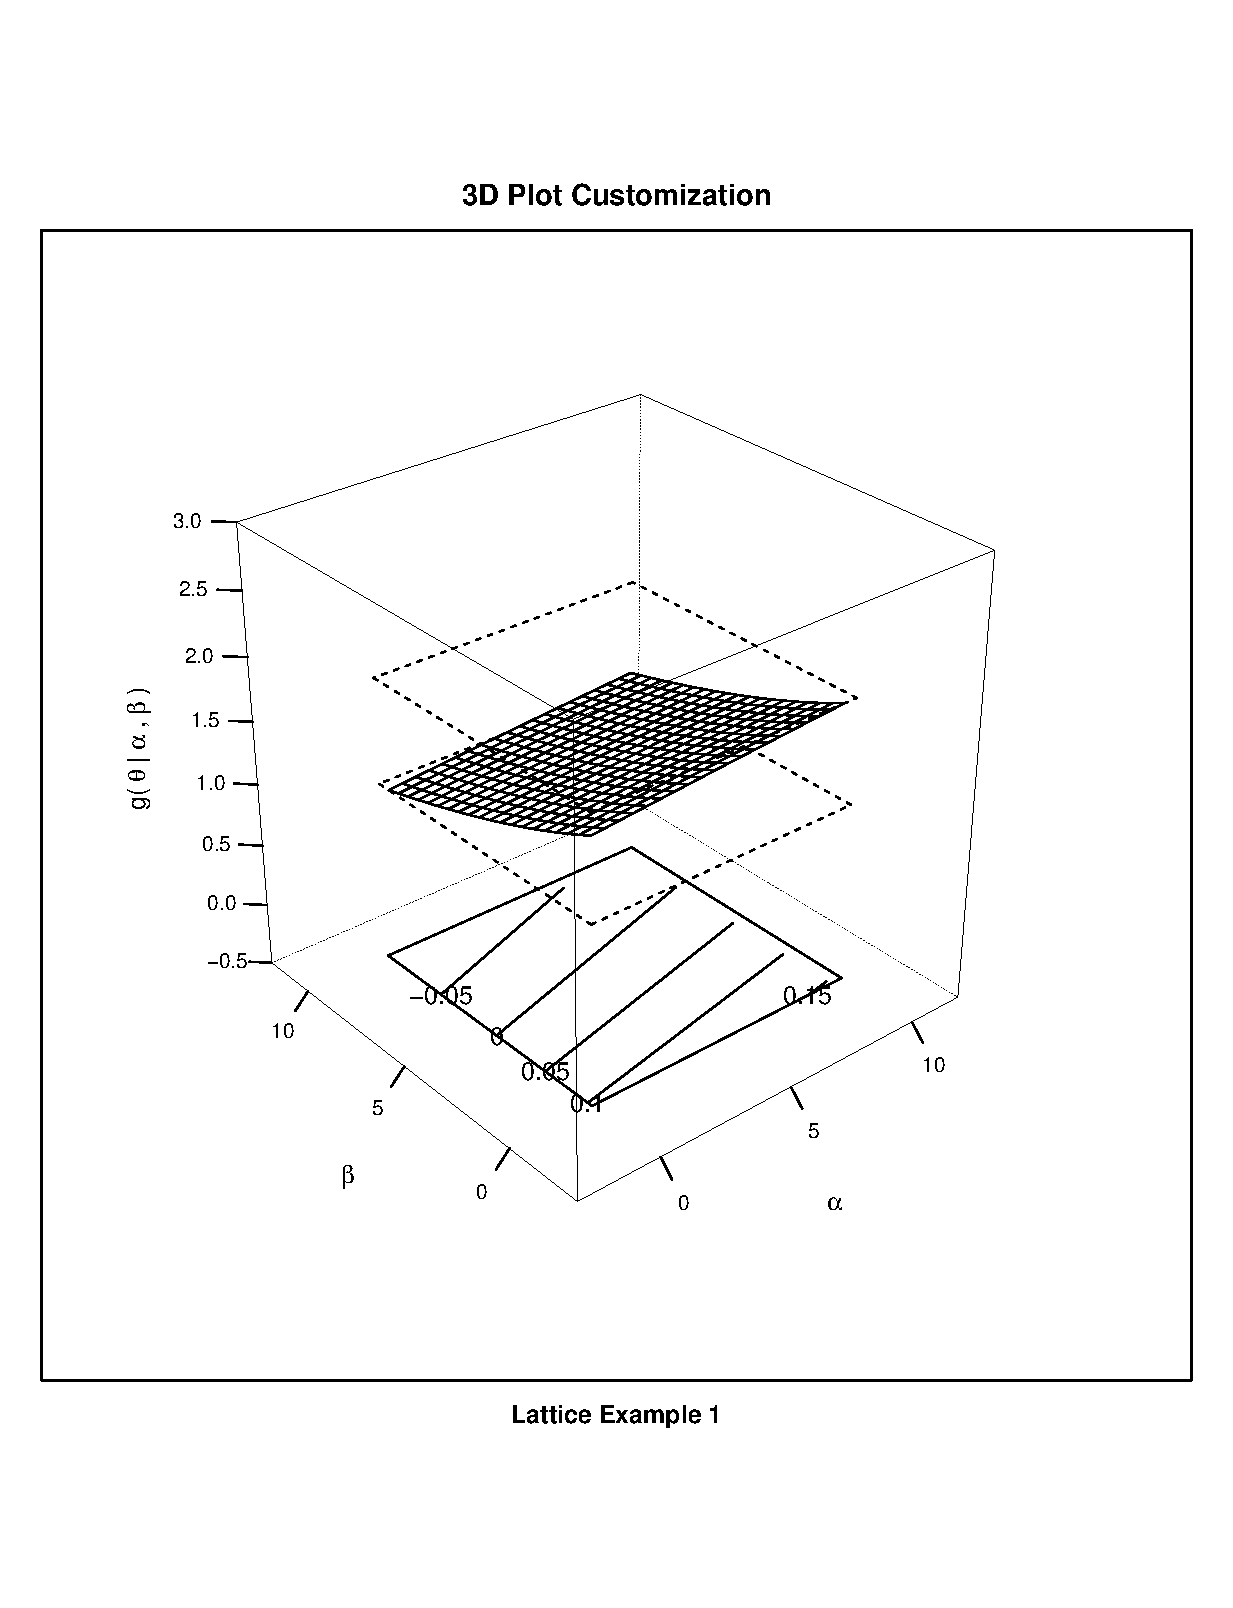
\includegraphics{./img/lattice-fig.eps}


\item \LaTeX 의 문서에 포함될 \texttt{.eps} 그래픽을 \texttt{R}에서 뽑았을 때는 아무런 문제가 없어 보였는데, 정작 \texttt{pdf}로 문서를 뽑아 보니까 이 그래픽이 들어간 페이지가 90도로 돌아가 있거나 혹은 그래픽이 90도로 회전되어 있을 경우에는 아래와 같이 하면 됩니다.

\begin{Schunk}
 \begin{Sinput}
  postscript(file=``filename.eps'', onefile=FALSE, horizontal=FALSE)
 \end{Sinput}
\end{Schunk}

이 문제에 대한 출처는 \texttt{postscript} 도움말입니다.

이문제를 다른 방법으로도 해결할 수 있습니다.  (대충 서너개 더 있음).

\item 새로운 그래픽 객체를 생성하는 방법을 설명해줘서 사용자가 추후에 독립적인 그래픽을 생성할 수 있게 도와주기 


	\item (접수: 2013-APR-23)  저는 다각형을 그리고 싶습니다. 
	
	\textsf{(답변)}  이것은 간단히 2차원-랜덤포인트 생성한 뒤에 \texttt{polygon()} 함수를 써서 보여주면 됨. 

\end{enumerate}

% ggplot2에서 stat_density2d에 오류가 있는것 같습니다. 모든 경우에 NA가 return된다는 보고




%%%%%%%%%%%%%%%%%%%%%%%%%%%%%%%%%%%%%%%%%%%%%%%%%%%%%%%%%%%%%%%%%%%%%%%%
%
% Utilities
%
%%%%%%%%%%%%%%%%%%%%%%%%%%%%%%%%%%%%%%%%%%%%%%%%%%%%%%%%%%%%%%%%%%%%%%%%

\part{분석 후의 패키지 개발}

\chapter{분석 후 개발과 관련하여}
\section{클래스와 메소드 그리고 패키지 제작}
\begin{enumerate}
\item 패키지를 만들고 싶어요. (흠.. Generalized Linear Model 프레임워크 흉내내서 똑같이 만들어보기 실습자료로 제공해주기)
\end{enumerate}
\begin{Schunk}
\begin{Soutput}
output
\end{Soutput}
\end{Schunk}



%%%%%%%%%%%%%%%%%%%%%%%%%%%%%%%%%%%%%%%%%%%%%%%%%%%%%%%%%%%%%%%%%%%%%%%%
%
% Miscellinous
%
%%%%%%%%%%%%%%%%%%%%%%%%%%%%%%%%%%%%%%%%%%%%%%%%%%%%%%%%%%%%%%%%%%%%%%%%


%%%%%%%%%%%%%%%%%%%%%%%%%%%%%%%%%%%%%%%%%%%%%%%%%%%%%%%%%%%%%%%%%%%%%%%%
%
%
%
%%%%%%%%%%%%%%%%%%%%%%%%%%%%%%%%%%%%%%%%%%%%%%%%%%%%%%%%%%%%%%%%%%%%%%%%

\section{간단한 GUI 제작 해보기}

\begin{enumerate}
	\item 다른 언어로 인터페이싱 하는 방법마로, 그냥 \texttt{R}에서 주어지는 패키지를 이용해서 간단한 GUI 환경만들기
	\item 아마도... R Commander를 확장하는 방법을 예로 들면 좋을 것 같음
	\item 원리도 간단히 설명해주면 더욱 좋을 것 같음. 
\end{enumerate}

\begin{Schunk}
\begin{Soutput}
output
\end{Soutput}
\end{Schunk}

%%%%%%%%%%%%%%%%%%%%%%%%%%%%%%%%%%%%%%%%%%%%%%%%%%%%%%%%%%%%%%%%%%%%%%%%
%
%
%
%%%%%%%%%%%%%%%%%%%%%%%%%%%%%%%%%%%%%%%%%%%%%%%%%%%%%%%%%%%%%%%%%%%%%%%%


\chapter{미분류 질문들}

% 콘솔 컨트롤
% ctrl + L을 누르면 콘솔의 내용이 모두 지워짐

이 섹션에 등록된 질문들은 접수만 되고 아직은 답변되지 않은 상태입니다
% http://www.columbia.edu/~cjd11/charles_dimaggio/DIRE/resources/R/rFunctionsList.pdf
% http://www.ats.ucla.edu/stat/r/library/advanced_function_r.htm
% http://www.sr.bham.ac.uk/~ajrs/R/r-function_list.html
% http://www.scidav.org/techno/r_environments


% 이런 느낌은 특히 최소한 내가 알기로는 경영학과 경제학 분야(거의 확실함) 및 사회학, 심리학 분야가 특히 심하다. 
% 그리고 이들 분야에서는
% R의 다양한 기능(특히 visualization) 또는 packages를 필요로 하지 않을 가능성이 높다. 왜냐하면 분석 방법이 단순하기 때문이다.
% 여기에서 분석 방법이 단순하다는 것은 그 이론적 배경이 쉽다는 것을 의미하는 것이 아니라 절차상의 얘기이다.
% 언급한 분야에서 학술연구에서 실행되는 분석의 양을 보면 대부분 [기술통계 - 상관관계 - 차이분석, 회귀분석, 구조방정식분석] 정도로
% 분석이 마무리 되기 때문이다. 그리고 대부분 표(table)로 결과를 보고하는 형식을 따르고 있다.
% 분석 모형 자체를 다루는 연구가 거의 없는 것이다. 따라서 R의 작업 방식은 그들에게는 불필요할 지도 모른다.

% 그러나 여전히 R의 다양한 source를 필요로 하는 아주 작은 규모의 학술연구 분야는 존재한다. 따라서 여기의 tips에는 이들을 고려하여
% R 사용에 도움이 될 만한 사항들을 정리하고자 한다.
% 개인적으로는 통계학 및 다른 분야의 연구 과정이 어떻게 진행되는지 잘 모르는 것도 한 몫하여 이에 해당하는 부분은 다른 이의 도움이
% 절실하다.

% 덧붙여 나는 윈도우 환경에서의 R tip에 주목하고자 한다(Mac이나 유닉스/리눅스 환경에서의 R 사용에 관한 tip도 다른 이의 도움이 필요한
% 부분이다). 그 이유는 내가 윈도우에서 SPSS와 SAS를 숙련시켜 왔기 때문에 대부분의 통계분석 초심자들도 윈도우 환경에서 R 을 접하게
% 될 것이라는 막연한 억측 때문이다. 시간이 지나면서 여러 사람들을 만나보게 꼭 그렇지만은 않다는 것을 알게 되었지만 최소한 경영학과
% 경제학 분야에 속한 사람들은 그럴 것이라는 확신 때문이다. 이것은 다른 분야의 사람들을 홀대하는 것이 아니라 나의 능력의 한계 때문이다.
% 실제로 나의 경우에도 최근에 C 언어, CentOS, 그리고 MySQL도 공부하기 시작했으니 오해는 하지 말기 바란다(누군가는 포기하라고도 했다.
% 왜냐하면 지금 그것들을 공부하기에는 분량이 너무 많고 난이도가 낮지 않기 때문이다). 그런데 결국에는 내 전공분야에서의 R 사용은
% 그 분량이 많지 않고 리눅스/유닉스 기반의 R 사용에 보다 많은 시간과 지면을 할애하게 될 것이라는 생각이 든다.

% R은 최근의 빅데이터라는 화두와 함께 큰 주목을 받고 있다. 하지만 대부분의 사람들, 특히 사회과학 전공자들은 이 개념적 정의도 제대로
% 알지 못하며 들어보지 못한  전문용어(SQL, Hadoop, 그리고 Mapreduce 등)에 혹하고 있는 실정이다.
% 나의 경우 R을 구글링(googling)으로 공부하였다. 왜냐하면 내가 재학하던 대학에서는 R 교육 프로그램이 없었기 때문이다. 처음 접하게 된
% 것은 미시경제분석 수업이었다. 그 수업에서 교수님이 수업을 진행하시는데 R을 사용한 것이다(SAS도 조금 사용했었으나 SPSS 는 잡동사니
% 취급을 하셨던 것으로 기억한다). 누군가에게 강의를 받는 식의 교육은 그것이 전부였다. 이후의 학습은 모두 맨땅에 해딩과 계란으로
% 바위깨기 식이었다. 이 R tips 과정은 이러한 어려움을 덜어주기 위한 방안이 될 수도 있을 것이다.
% 그러기를 한참 후 어느 정도 익숙해지고 나니, 또 연구자로서의 건방이 살아나 R 교육이 어떻게 이루어지고 있는 지가 궁금해졌다.
% 이 부분은 나중에 다시 써 볼라오,,,


\begin{enumerate}
	
% 아래의 주소로부터 질문 다 만들어내기 	
% http://www.statmethods.net/input/valuelabels.html


	\item (접수: 2013-APR-23)  제가 가진 데이터셋이 있는데, 이 데이터를 어떤 특정한 변수들의 값을 이용하여 분류하려고 합니다.  어떻게 해야하나요?
	
	\textsf{(답변)}  요것은 \texttt{split()} 함수를 이용하도록 알려줄 것. 

	\item (접수: 2013-APR-23) 제가 가진 데이터 프레임에 NA 값들이 있는데, NA 때문에 분석이 이상해지는 것 같아, NA를 가진 데이터 행자체를 없애고 싶습니다.  한번에 해주는게 없나요? 
	
	\textsf{(답변)}  요건 \texttt{na.omit()}과 같은 함수를 이용하는 법을 알려줄 것.  흠.. \texttt{na.action}이라는 개념을 알려주면 더욱 좋음. 

	\item (접수: 2013-APR-23) 논리형 벡터가 있는데, 이 벡터의 구성요소가 모두 TRUE 인지 알고 싶습니다. 
	
	\textsf{(답변)} 이건 \texttt{isTRUE()}함수와 \texttt{all()}함수를 통해 알려주면 매우 좋음.
		
	\item (접수: 2013-APR-22) 선형방정식 $AX=b$의 해 $X$를 찾으려면 어떻게 해야 하나요? 
	
	\textsf{(답변)} \texttt{solve()} 함수의 사용법을 알려줄 것.
	
	\item (접수: 2013-APR-21) R 패키지를 CRAN에 올리는 방법을 알려주세요 
	
	\textsf{(답변)} 이 질문을 대답할 때는 반드시 CRAN Package Submission Guideline에 대해서 알려줘야 함.  (이거 번역해 놨는데 당췌 어디에 뒀는지 찾을 수가 없음, 2013-04-20 까지 못 찾으면 새로이 번역할 것)
	
	\item (접수: 2013-APR-19) R은 처음부터 기존의 통계팩키지와는 다른 모습에 약간 두렵기까지 합니다.  기존의 분석은 일반적으로 $[$프로그램 실행 $->$ 데이터 불러오기 $->$ 분석(메뉴클릭:SPSS 또는 명령어입력:SAS) $->$ 실행$]$의 절차를 밟아 왔기에 모든 결과를 한 번에 보여주는 식입니다. 그러나 R은 그렇지 않아 이러한 점부터 생소하고 이상합니다.  데이터를 불러오기 하면 바로 데이터시트를 볼 수 있는 것도 아닙니다 (접수날짜: 2013-APR-17).

	\item (접수: 2013-04-18, Reproducibility=NO) read.xlsx함수를 이용해 xlsx파일에서 데이터프레임형태로 가져옵니다. 이 때 [3,3] 셀에 있는 텍스트가 "3월" 이라고 할 때 temp[3,3] == "3월" 이렇게 비교하려고 하면 제대로 비교가 안되더군요.. 한글 텍스트로 이루어진 변수값를 비교하는 방법이 어떤게 있는지 궁금합니다.
	
	\item 분석을 하고 나면 결과를 그래프나 그림으로 나타내게 되는데 R에서는 그림을 나타내는 창이 하나만 나타나서 동시에 두 개를 보지 못하는 경우가 허다한데, 이의 해결방법은 없나요? (접수: 2013-APR-13, 분류: 그래픽스 관련) 
	
	\textsf{(답변)} \texttt{R}에서는 그래픽 디바이스가 그래픽 생성시 마다 초기화되어 다시 보여줌으로서 그래픽 창이 하나만 계속 보여지는 것입니다.  새로운 그래프를 또다른 장치를 통해 보여주고자 한다면 \texttt{X11()}이라는 명령어를 이용하면 됩니다.  
	이 명령어는 유닉스환경에 설치된 \texttt{R}의 경우에 해당합니다.  
	


\end{enumerate}


\section{답변되지 않을 수도 있는 질문들}

\begin{enumerate}
	\item (접수: 2013-04-18, Reproducibility=NA) R의 장점이자 단점이라고 생각되는 것 중에 하나가 엄청난 수의 패키지들임. 즉 어떤 분석을 하고자 할 때 그것에 대해 하나의 패키지가 있는 것이 아니라 대체적으로 사용가능한 패키지들이 존재하는데 이들 중 어느 것을 써야할 지 잘 모름. 다른 분석 프로그램의 경우 이러한 문제가 없는데... 결국엔 어떻게 제일 성능이 좋은? 결과가 신뢰할 만한? 좋은 패키지를 선택하는가를 알려주었으면 좋겠씀돠.
	
	\textsf{(답변)} 이것은 경험에 해당되며, 해당분야의 전문가로부터의 조언을 받는 것이 안전합니다.  그렇지 않다면, 직접 베이스를 이용하여 작성하면 됩니다. 
	
\end{enumerate}

% R을 사용해서 web 크롤링을 하는데 속도가 엄청 느리네요 scan() 함수를 쓰면 url로부터 html데이터를 받게 되는데 이것을 substring()함수와 regexprs()함수를 사용하여 적절히 데이터를 분해 하는 작업을 하는데 엄청느리네요. 원체느린거 같은데 혹시 해결방안 아시는분 게시나요?

% R에 있는 ggplot2 패키지를 이용해 얻은 얻은 plot그림을 웹에 보여주는 방법에 대해 아시는 분 계신가요?


\part{알면 도움이 되는}
\chapter{유닉스 명령어}

\chapter{\LaTeX 사용법}

\chapter{Perl 명령어}

\chapter{C 언어} 


\nocite{GNUR}
\nocite{GNUR-FAQ}

\bibliographystyle{apalike}
\bibliography{tutorial}

\end{document}

% CRAN Repository Policy  -- http://cran.r-project.org/web/packages/policies.html 


% Useful documents
% An Introduction to the interactive debugging tools in R, Roger, D. Peng, UCLA, 
% R Guide: March 2011, L. Chihara 
% Statistical Analysis with R - a quick start - Oleg Nenadic, Walter Zucchini September 2004
% R Package writing tutorial - Harvard Statistics, Alan Lenarcic, August 28, 2007
% Graphical User Interface - http://www.stat.berkely.edu/classes/s244/gui/Gui1.html 
% GUI Development with tcl/tk -- http://wwww.sciviews.org/_rgui/tcltk/Mb.html 
% Interactive 3D plots with the rgl package http://casoilresource.lawr.ucdavis.edu/drupal/node/371 
% Exploring data with statistical graphices in R, Duncan Murdoch, Nov 23 2011, 
% An R-library for 3D visualization with OpenGL, oleg Nenadic, Daniel Adler, Walter Zucchini 
% Advanced Graphics with R, universitat de Barcelona, April 30, 2009. 
% STAT 846 Computational Techniques in Statistics Lecture Notes Longhai 
